\documentclass[twoside]{book}

% Packages required by doxygen
\usepackage{calc}
\usepackage{doxygen}
\usepackage{graphicx}
\usepackage[utf8]{inputenc}
\usepackage{makeidx}
\usepackage{multicol}
\usepackage{multirow}
\usepackage{textcomp}
\usepackage[table]{xcolor}

% Font selection
\usepackage[T1]{fontenc}
\usepackage{mathptmx}
\usepackage[scaled=.90]{helvet}
\usepackage{courier}
\usepackage{amssymb}
\usepackage{sectsty}
\renewcommand{\familydefault}{\sfdefault}
\allsectionsfont{%
  \fontseries{bc}\selectfont%
  \color{darkgray}%
}
\renewcommand{\DoxyLabelFont}{%
  \fontseries{bc}\selectfont%
  \color{darkgray}%
}

% Page & text layout
\usepackage{geometry}
\geometry{%
  a4paper,%
  top=2.5cm,%
  bottom=2.5cm,%
  left=2.5cm,%
  right=2.5cm%
}
\tolerance=750
\hfuzz=15pt
\hbadness=750
\setlength{\emergencystretch}{15pt}
\setlength{\parindent}{0cm}
\setlength{\parskip}{0.2cm}
\makeatletter
\renewcommand{\paragraph}{%
  \@startsection{paragraph}{4}{0ex}{-1.0ex}{1.0ex}{%
    \normalfont\normalsize\bfseries\SS@parafont%
  }%
}
\renewcommand{\subparagraph}{%
  \@startsection{subparagraph}{5}{0ex}{-1.0ex}{1.0ex}{%
    \normalfont\normalsize\bfseries\SS@subparafont%
  }%
}
\makeatother

% Headers & footers
\usepackage{fancyhdr}
\pagestyle{fancyplain}
\fancyhead[LE]{\fancyplain{}{\bfseries\thepage}}
\fancyhead[CE]{\fancyplain{}{}}
\fancyhead[RE]{\fancyplain{}{\bfseries\leftmark}}
\fancyhead[LO]{\fancyplain{}{\bfseries\rightmark}}
\fancyhead[CO]{\fancyplain{}{}}
\fancyhead[RO]{\fancyplain{}{\bfseries\thepage}}
\fancyfoot[LE]{\fancyplain{}{}}
\fancyfoot[CE]{\fancyplain{}{}}
\fancyfoot[RE]{\fancyplain{}{\bfseries\scriptsize Generated on Wed Apr 13 2016 23\-:01\-:01 for srcl\-\_\-ctrl\-: planning by Doxygen }}
\fancyfoot[LO]{\fancyplain{}{\bfseries\scriptsize Generated on Wed Apr 13 2016 23\-:01\-:01 for srcl\-\_\-ctrl\-: planning by Doxygen }}
\fancyfoot[CO]{\fancyplain{}{}}
\fancyfoot[RO]{\fancyplain{}{}}
\renewcommand{\footrulewidth}{0.4pt}
\renewcommand{\chaptermark}[1]{%
  \markboth{#1}{}%
}
\renewcommand{\sectionmark}[1]{%
  \markright{\thesection\ #1}%
}

% Indices & bibliography
\usepackage{natbib}
\usepackage[titles]{tocloft}
\setcounter{tocdepth}{3}
\setcounter{secnumdepth}{5}
\makeindex

% Hyperlinks (required, but should be loaded last)
\usepackage{ifpdf}
\ifpdf
  \usepackage[pdftex,pagebackref=true]{hyperref}
\else
  \usepackage[ps2pdf,pagebackref=true]{hyperref}
\fi
\hypersetup{%
  colorlinks=true,%
  linkcolor=blue,%
  citecolor=blue,%
  unicode%
}

% Custom commands
\newcommand{\clearemptydoublepage}{%
  \newpage{\pagestyle{empty}\cleardoublepage}%
}


%===== C O N T E N T S =====

\begin{document}

% Titlepage & ToC
\hypersetup{pageanchor=false}
\pagenumbering{roman}
\begin{titlepage}
\vspace*{7cm}
\begin{center}%
{\Large srcl\-\_\-ctrl\-: planning }\\
\vspace*{1cm}
{\large Generated by Doxygen 1.8.6}\\
\vspace*{0.5cm}
{\small Wed Apr 13 2016 23:01:01}\\
\end{center}
\end{titlepage}
\clearemptydoublepage
\tableofcontents
\clearemptydoublepage
\pagenumbering{arabic}
\hypersetup{pageanchor=true}

%--- Begin generated contents ---
\chapter{Main Page}
\label{index}\hypertarget{index}{}\subsection*{Overview}

The working environment of a robot is usually represented as a map. To find a path for the robot to traverse the environment, we need to extract information from the map and use proper data structures to represent the workspace. A variety of approaches have been proposed by researchers to find a path from the workspace which can satisfy specified requirements.

\subsubsection*{1. Planning Based on Discrete Search}

The workspace can be represented by smaller, connected areas so that discrete search algorithms can be used for path planning. As shown in the following figure, one needs to choose a proper method to decompose the workspace first and then use a graph to represent the pairwise relations between neighbour areas. With the graph, algorithms like A$\ast$ can be performed to find a sequence of areas that connects the starting and finishing points.

 Currently there are two methods provided to decompose the workspace\-: square grid and quadtree.

\subsubsection*{2. Sample-\/\-Based Motion Planning}

\subsection*{Modules}


\begin{DoxyItemize}
\item Square grid
\item Quadtree
\item \hyperlink{graph}{Graph}
\end{DoxyItemize}

\subsection*{Known Issues}


\begin{DoxyItemize}
\item (Solved) A$\ast$ search algorithm currently only works with nodes that have attribute \char`\"{}location\-\_\-\char`\"{}. This attribute is used to calculate heuristic cost. A more general method may need to be implemented in the future. 
\end{DoxyItemize}
\chapter{Graph}
\label{graph}
\hypertarget{graph}{}
\subsubsection*{a. Design}

Graph is a type of data structure that can be used to represent pairwise relations between objects. In this library, a graph is modeled as a collection of vertices and edges. The relations between those concepts are shown as follows.
\begin{DoxyItemize}
\item Graph
\begin{DoxyItemize}
\item Vertex 1
\begin{DoxyItemize}
\item Edge 1\-\_\-1
\item Edge 1\-\_\-2
\item ...
\end{DoxyItemize}
\item Vertex 2
\begin{DoxyItemize}
\item Edge 2\-\_\-1
\item Edge 2\-\_\-2
\item ...
\end{DoxyItemize}
\item ...
\item Vertex n
\begin{DoxyItemize}
\item Edge n\-\_\-1
\item Edge n\-\_\-2
\item ...
\item Edge n\-\_\-m
\end{DoxyItemize}
\end{DoxyItemize}
\end{DoxyItemize}

A minimal implementation of Graph consists of a list of vertices, each of which has an unique I\-D and a list of edges. For path finding in the graph, we need to add extra attributes, such as edge cost in Edge and heuristics, flags in Vertex for A$\ast$ search. These attributes are generic for all graphs.

In different contexts, we usually want to add non-\/generic attributes to the vertex so that it can be meaningful for the application. For example when we use a graph to represent a square grid, a square cell can be regarded as a vertex, and the connectivities of a cell with its neighbour cells can be represented as edges. In this case, a square cell (vertex) may have attributes such as its location in the grid and its occupancy type (cell filled with obstacle or not). Such attributes can be very different across different applications, thus they are not modeled directly in the \char`\"{}\-Vertex\char`\"{} data structure. Instead, the \char`\"{}additional information\char`\"{} is packed into a separate object (called a {\bfseries Bundled Data Structure (B\-D\-S)} in this design) and we associate a bundled data structure with a vertex uniquely.

\subsubsection*{b. Implementation}

There are 3 class templates defined\-: {\bfseries Graph}, {\bfseries Vertex}, {\bfseries Edge}. The use of template enables us to associate different types of \char`\"{}\-B\-D\-S\char`\"{} to a vertex, without modifying the code of the aforementioned 3 classes. In other words, the Graph, Vertex and Edge all have a \char`\"{}type\char`\"{}, which is determined by the type of B\-D\-S we want to associate with the vertex. With the current implementation, the B\-D\-S has to be defined as a class or struct. {\bfseries A user-\/defined B\-D\-S class/struct has to inherit from B\-D\-S\-Base class before we use them to construct a graph.} In the graph data structure, the vertex has the same I\-D with the B\-D\-S it's associated with. This is for solely for easy indexing to find one with the other.

Here is an example to use the templates.

I. We first define a B\-D\-S type we want to use for constructing the graph.


\begin{DoxyCode}
\textcolor{keyword}{struct }BDSExample: \textcolor{keyword}{public} BDSBase<BDSExample>
\{
    BDSExample(uint64\_t \textcolor{keywordtype}{id}):
        BDSBase<BDSExample>(id)\{\};
    ~BDSExample()\{\};

    \textcolor{comment}{// simplest implementation of the function}
    \textcolor{keywordtype}{double} GetHeuristic(\textcolor{keyword}{const} BDSExample& other\_struct)\textcolor{keyword}{ const }\{
        \textcolor{keywordflow}{return} 0.0;
    \}
\};
\end{DoxyCode}


I\-I. Then we can create a few objects of class B\-D\-S\-Example


\begin{DoxyCode}
std::vector<BDSExample*> nodes;

\textcolor{comment}{// create nodes to be bundled with the graph vertices}
\textcolor{keywordflow}{for}(\textcolor{keywordtype}{int} i = 0; i < 9; i++) \{
    nodes.push\_back(\textcolor{keyword}{new} BDSExample(i));
\end{DoxyCode}


I\-I\-I. Now use those nodes to construct a graph. Note that the graph is of type B\-D\-S\-Example in this example.


\begin{DoxyCode}
\textcolor{comment}{// create a graph}
Graph<BDSExample> graph;

\textcolor{comment}{// the reference is used to access the bundled data structure in a vertex,}
\textcolor{comment}{//  so you need to pass in an object instead of a pointer}
graph.AddEdge(*(nodes[0]), *(nodes[1]), 1.0);
graph.AddEdge(*(nodes[0]), *(nodes[2]), 1.5);
graph.AddEdge(*(nodes[1]), *(nodes[2]), 2.0);
graph.AddEdge(*(nodes[2]), *(nodes[3]), 2.5);
\end{DoxyCode}


I\-V. Now you've got a graph. You can print all edges of this graph in the following way


\begin{DoxyCode}
\textcolor{keyword}{auto} all\_edges = graph.GetGraphEdges();

\textcolor{keywordflow}{for}(\textcolor{keyword}{auto} e : all\_edges)
    e.PrintEdge();
\end{DoxyCode}


You will get the output


\begin{DoxyCode}
Edge: start - 0 , end - 1 , cost - 1
Edge: start - 0 , end - 2 , cost - 1.5
Edge: start - 1 , end - 2 , cost - 2
Edge: start - 2 , end - 3 , cost - 2.5
\end{DoxyCode}


\subsubsection*{c. Memory Management}

When a Graph object goes out of scope, its destructor function will recycle memory allocated for this its vertices and edges. However, {\bfseries the graph doesn't recycle memory allocated for the bundled data structure that each vertex is associated with}. In the square grid example, the graph doesn't assume the square grid also becomes useless when the graph itself is destructed. The {\bfseries square grid} should be responsible for recycling the memory allocated for its square cells when it becomes of no use. Thus in the above simple example, we will need to do the following operation to free the memory at the end.


\begin{DoxyCode}
\textcolor{comment}{// delete objects of BDSExample}
\textcolor{keywordflow}{for}(\textcolor{keyword}{auto}& e : nodes)
        \textcolor{keyword}{delete} e;
\end{DoxyCode}


\subsubsection*{d. Notes on Graph}


\begin{DoxyItemize}
\item You may have noticed that when constructing a graph, you don't need to explicitly create objects of \char`\"{}\-Vertex\char`\"{}. By calling member function {\bfseries Add\-Edge(src\-\_\-node, dst\-\_\-node, cost)} of the graph, vertices are created and associated with the according B\-D\-S internally.
\item There are two views of the graph data structure. When constructing the graph (bottom-\/up view), the B\-D\-Ss are manipulated directly and vertices are handled implicitly. When using the graph (top-\/down view) for path search, vertices are the the entities you're directly interacting with and the B\-D\-Ss they associate with are probably of less interest. Of course, you can access one from the other easily using their common I\-D.
\item A$\ast$ performs search on Vertex objects, so the A$\ast$ algorithm also has a \char`\"{}type\char`\"{}. In this implementation, A$\ast$ search is provided as a member function of Graph. So you don't need to explicitly declare and initialize an A$\ast$ instance. You can simply perform search on a graph by calling the search function packed in the graph.
\item An detailed example of using the graph for path search can be found in \char`\"{}apps/example.\-cpp\char`\"{}. The work flow is shown as follows.
\end{DoxyItemize}


\begin{DoxyCode}
\textcolor{comment}{// create a graph from square grid}
Graph<SquareCell>* graph = GraphBuilder::BuildFromSquareGrid(grid,\textcolor{keyword}{true});

\textcolor{comment}{// specify search start and finish vertex}
Vertex<SquareCell>* start\_vertex = graph->GetVertexFromID(0);
Vertex<SquareCell>* finish\_vertex = graph->GetVertexFromID(1);

\textcolor{comment}{// perform A* search and get a vector of Vertics as the search result}
std::vector<Vertex<SquareCell>*> path = graph->AStarSearch(start\_vertex,finish\_vertex);
\end{DoxyCode}
 
\chapter{Known Issues}
\label{known_issues}
\hypertarget{known_issues}{}

\begin{DoxyItemize}
\item A$\ast$ search algorithm currently only works with nodes that have attribute \char`\"{}location\-\_\-\char`\"{}. This attribute is used to calculate heuristic cost. A more general method may need to be implemented in the future. 
\end{DoxyItemize}
\chapter{R\-E\-A\-D\-M\-E}
\label{md__home_rdu_Workspace_srcl_robot_suite_srcl_ctrl_planning_src_graph_README}
\hypertarget{md__home_rdu_Workspace_srcl_robot_suite_srcl_ctrl_planning_src_graph_README}{}
Reference\-:

Graph


\begin{DoxyItemize}
\item \href{http://www.geeksforgeeks.org/graph-and-its-representations/}{\tt http\-://www.\-geeksforgeeks.\-org/graph-\/and-\/its-\/representations/}
\item \href{https://www.topcoder.com/community/data-science/data-science-tutorials/power-up-c-with-the-standard-template-library-part-1/}{\tt https\-://www.\-topcoder.\-com/community/data-\/science/data-\/science-\/tutorials/power-\/up-\/c-\/with-\/the-\/standard-\/template-\/library-\/part-\/1/}
\item \href{https://www.topcoder.com/community/data-science/data-science-tutorials/power-up-c-with-the-standard-template-library-part-2/}{\tt https\-://www.\-topcoder.\-com/community/data-\/science/data-\/science-\/tutorials/power-\/up-\/c-\/with-\/the-\/standard-\/template-\/library-\/part-\/2/}
\item \href{http://stackoverflow.com/questions/17473753/c11-return-value-optimization-or-move/17473869#17473869}{\tt http\-://stackoverflow.\-com/questions/17473753/c11-\/return-\/value-\/optimization-\/or-\/move/17473869\#17473869}
\item \href{http://lafstern.org/matt/col1.pdf}{\tt http\-://lafstern.\-org/matt/col1.\-pdf}
\end{DoxyItemize}

Search


\begin{DoxyItemize}
\item \href{http://homepages.abdn.ac.uk/f.guerin/pages/teaching/CS1013/practicals/aStarTutorial.htm}{\tt http\-://homepages.\-abdn.\-ac.\-uk/f.\-guerin/pages/teaching/\-C\-S1013/practicals/a\-Star\-Tutorial.\-htm}
\item \href{http://www.cppblog.com/mythit/archive/2009/04/19/80492.aspx}{\tt http\-://www.\-cppblog.\-com/mythit/archive/2009/04/19/80492.\-aspx} (Chinese Version)
\item \href{http://users.cis.fiu.edu/~weiss/adspc++2/code/}{\tt http\-://users.\-cis.\-fiu.\-edu/$\sim$weiss/adspc++2/code/}
\item \href{http://heyes-jones.com/astar.php}{\tt http\-://heyes-\/jones.\-com/astar.\-php}
\item \href{http://stackoverflow.com/questions/11912736/c-a-star-implementation-determining-whether-a-node-is-already-in-the-priori}{\tt http\-://stackoverflow.\-com/questions/11912736/c-\/a-\/star-\/implementation-\/determining-\/whether-\/a-\/node-\/is-\/already-\/in-\/the-\/priori}
\item \href{http://stackoverflow.com/questions/10394508/which-std-container-to-use-in-a-algorithms-openset}{\tt http\-://stackoverflow.\-com/questions/10394508/which-\/std-\/container-\/to-\/use-\/in-\/a-\/algorithms-\/openset}
\item \href{https://github.com/justinhj/astar-algorithm-cpp}{\tt https\-://github.\-com/justinhj/astar-\/algorithm-\/cpp}
\item \href{http://code.activestate.com/recipes/577457-a-star-shortest-path-algorithm/}{\tt http\-://code.\-activestate.\-com/recipes/577457-\/a-\/star-\/shortest-\/path-\/algorithm/}
\item \href{http://theory.stanford.edu/~amitp/GameProgramming/}{\tt http\-://theory.\-stanford.\-edu/$\sim$amitp/\-Game\-Programming/}
\end{DoxyItemize}

C++


\begin{DoxyItemize}
\item \href{http://stackoverflow.com/questions/642229/why-do-i-need-to-use-typedef-typename-in-g-but-not-vs}{\tt http\-://stackoverflow.\-com/questions/642229/why-\/do-\/i-\/need-\/to-\/use-\/typedef-\/typename-\/in-\/g-\/but-\/not-\/vs}
\item \href{http://stackoverflow.com/questions/8584431/why-is-the-keyword-typename-needed-before-qualified-dependent-names-and-not-b}{\tt http\-://stackoverflow.\-com/questions/8584431/why-\/is-\/the-\/keyword-\/typename-\/needed-\/before-\/qualified-\/dependent-\/names-\/and-\/not-\/b} 
\end{DoxyItemize}
\chapter{Namespace Index}
\section{Namespace List}
Here is a list of all namespaces with brief descriptions\-:\begin{DoxyCompactList}
\item\contentsline{section}{\hyperlink{namespacesrcl__ctrl}{srcl\-\_\-ctrl} }{\pageref{namespacesrcl__ctrl}}{}
\end{DoxyCompactList}

\chapter{Class Index}
\section{Class List}
Here are the classes, structs, unions and interfaces with brief descriptions\-:\begin{DoxyCompactList}
\item\contentsline{section}{\hyperlink{classsrcl__ctrl_1_1AStar}{srcl\-\_\-ctrl\-::\-A\-Star$<$ Graph\-Vertex\-Type $>$} \\*A$\ast$ search algorithm }{\pageref{classsrcl__ctrl_1_1AStar}}{}
\item\contentsline{section}{\hyperlink{classsrcl__ctrl_1_1Edge}{srcl\-\_\-ctrl\-::\-Edge$<$ Edge\-Vertex\-Type $>$} \\*An edge data structure template }{\pageref{classsrcl__ctrl_1_1Edge}}{}
\item\contentsline{section}{\hyperlink{structsrcl__ctrl_1_1ExampleNode}{srcl\-\_\-ctrl\-::\-Example\-Node} \\*An example node that can be associated with a vertex }{\pageref{structsrcl__ctrl_1_1ExampleNode}}{}
\item\contentsline{section}{\hyperlink{classsrcl__ctrl_1_1Graph}{srcl\-\_\-ctrl\-::\-Graph$<$ Graph\-Node\-Type $>$} \\*A graph data structure template }{\pageref{classsrcl__ctrl_1_1Graph}}{}
\item\contentsline{section}{\hyperlink{structsrcl__ctrl_1_1PriorityQueue}{srcl\-\_\-ctrl\-::\-Priority\-Queue$<$ T, Number $>$} \\*A simple priority queue structure used as A$\ast$ open list }{\pageref{structsrcl__ctrl_1_1PriorityQueue}}{}
\item\contentsline{section}{\hyperlink{classsrcl__ctrl_1_1Vertex}{srcl\-\_\-ctrl\-::\-Vertex$<$ Vertex\-Node\-Type $>$} \\*A vertex data structure template }{\pageref{classsrcl__ctrl_1_1Vertex}}{}
\end{DoxyCompactList}

\chapter{File Index}
\section{File List}
Here is a list of all files with brief descriptions\-:\begin{DoxyCompactList}
\item\contentsline{section}{/home/rdu/\-Workspace/srcl\-\_\-robot\-\_\-suite/srcl\-\_\-ctrl/planning/src/graph/\hyperlink{astar_8h}{astar.\-h} }{\pageref{astar_8h}}{}
\item\contentsline{section}{/home/rdu/\-Workspace/srcl\-\_\-robot\-\_\-suite/srcl\-\_\-ctrl/planning/src/graph/\hyperlink{graph_8h}{graph.\-h} }{\pageref{graph_8h}}{}
\item\contentsline{section}{/home/rdu/\-Workspace/srcl\-\_\-robot\-\_\-suite/srcl\-\_\-ctrl/planning/src/graph/\hyperlink{vertex_8h}{vertex.\-h} }{\pageref{vertex_8h}}{}
\end{DoxyCompactList}

\chapter{Namespace Documentation}
\hypertarget{namespacesrcl__ctrl}{\section{srcl\-\_\-ctrl Namespace Reference}
\label{namespacesrcl__ctrl}\index{srcl\-\_\-ctrl@{srcl\-\_\-ctrl}}
}
\subsection*{Classes}
\begin{DoxyCompactItemize}
\item 
struct \hyperlink{structsrcl__ctrl_1_1PriorityQueue}{Priority\-Queue}
\begin{DoxyCompactList}\small\item\em A simple priority queue structure used as A$\ast$ open list. \end{DoxyCompactList}\item 
class \hyperlink{classsrcl__ctrl_1_1AStar}{A\-Star}
\begin{DoxyCompactList}\small\item\em A$\ast$ search algorithm. \end{DoxyCompactList}\item 
class \hyperlink{classsrcl__ctrl_1_1BDSBase}{B\-D\-S\-Base}
\begin{DoxyCompactList}\small\item\em The base class of bundled data structure. \end{DoxyCompactList}\item 
struct \hyperlink{structsrcl__ctrl_1_1BDSExample}{B\-D\-S\-Example}
\begin{DoxyCompactList}\small\item\em An example B\-D\-S that can be associated with a vertex. \end{DoxyCompactList}\item 
class \hyperlink{classsrcl__ctrl_1_1Graph}{Graph}
\begin{DoxyCompactList}\small\item\em A graph data structure template. \end{DoxyCompactList}\item 
class \hyperlink{classsrcl__ctrl_1_1Edge}{Edge}
\begin{DoxyCompactList}\small\item\em An edge data structure template. \end{DoxyCompactList}\item 
class \hyperlink{classsrcl__ctrl_1_1Vertex}{Vertex}
\begin{DoxyCompactList}\small\item\em A vertex data structure template. \end{DoxyCompactList}\end{DoxyCompactItemize}

\chapter{Class Documentation}
\hypertarget{classsrcl__ctrl_1_1AStar}{\section{srcl\-\_\-ctrl\-:\-:A\-Star$<$ Graph\-Vertex\-Type $>$ Class Template Reference}
\label{classsrcl__ctrl_1_1AStar}\index{srcl\-\_\-ctrl\-::\-A\-Star$<$ Graph\-Vertex\-Type $>$@{srcl\-\_\-ctrl\-::\-A\-Star$<$ Graph\-Vertex\-Type $>$}}
}


A$\ast$ search algorithm.  




{\ttfamily \#include $<$astar.\-h$>$}

\subsection*{Public Member Functions}
\begin{DoxyCompactItemize}
\item 
\hyperlink{classsrcl__ctrl_1_1AStar_a449cf8eefb93e6ddab1d821c52af76e2}{A\-Star} ()
\item 
\hyperlink{classsrcl__ctrl_1_1AStar_a27601d7fd7e9608a333e26e9ba31453a}{$\sim$\-A\-Star} ()
\item 
std\-::vector$<$ Graph\-Vertex\-Type $\ast$ $>$ \hyperlink{classsrcl__ctrl_1_1AStar_afe487e5443813c4a238b745bd2d73a9b}{Search} (Graph\-Vertex\-Type $\ast$start, Graph\-Vertex\-Type $\ast$goal)
\end{DoxyCompactItemize}
\subsection*{Private Member Functions}
\begin{DoxyCompactItemize}
\item 
double \hyperlink{classsrcl__ctrl_1_1AStar_a0a4b0df9a4b80bc65856e81132c179a7}{Calc\-Heuristic} (Graph\-Vertex\-Type $\ast$vertex\-\_\-a, Graph\-Vertex\-Type $\ast$vertex\-\_\-b)
\end{DoxyCompactItemize}


\subsection{Detailed Description}
\subsubsection*{template$<$typename Graph\-Vertex\-Type$>$class srcl\-\_\-ctrl\-::\-A\-Star$<$ Graph\-Vertex\-Type $>$}

A$\ast$ search algorithm. 

\subsection{Constructor \& Destructor Documentation}
\hypertarget{classsrcl__ctrl_1_1AStar_a449cf8eefb93e6ddab1d821c52af76e2}{\index{srcl\-\_\-ctrl\-::\-A\-Star@{srcl\-\_\-ctrl\-::\-A\-Star}!A\-Star@{A\-Star}}
\index{A\-Star@{A\-Star}!srcl_ctrl::AStar@{srcl\-\_\-ctrl\-::\-A\-Star}}
\subsubsection[{A\-Star}]{\setlength{\rightskip}{0pt plus 5cm}template$<$typename Graph\-Vertex\-Type$>$ {\bf srcl\-\_\-ctrl\-::\-A\-Star}$<$ Graph\-Vertex\-Type $>$\-::{\bf A\-Star} (
\begin{DoxyParamCaption}
{}
\end{DoxyParamCaption}
)\hspace{0.3cm}{\ttfamily [inline]}}}\label{classsrcl__ctrl_1_1AStar_a449cf8eefb93e6ddab1d821c52af76e2}
\hypertarget{classsrcl__ctrl_1_1AStar_a27601d7fd7e9608a333e26e9ba31453a}{\index{srcl\-\_\-ctrl\-::\-A\-Star@{srcl\-\_\-ctrl\-::\-A\-Star}!$\sim$\-A\-Star@{$\sim$\-A\-Star}}
\index{$\sim$\-A\-Star@{$\sim$\-A\-Star}!srcl_ctrl::AStar@{srcl\-\_\-ctrl\-::\-A\-Star}}
\subsubsection[{$\sim$\-A\-Star}]{\setlength{\rightskip}{0pt plus 5cm}template$<$typename Graph\-Vertex\-Type$>$ {\bf srcl\-\_\-ctrl\-::\-A\-Star}$<$ Graph\-Vertex\-Type $>$\-::$\sim${\bf A\-Star} (
\begin{DoxyParamCaption}
{}
\end{DoxyParamCaption}
)\hspace{0.3cm}{\ttfamily [inline]}}}\label{classsrcl__ctrl_1_1AStar_a27601d7fd7e9608a333e26e9ba31453a}


\subsection{Member Function Documentation}
\hypertarget{classsrcl__ctrl_1_1AStar_a0a4b0df9a4b80bc65856e81132c179a7}{\index{srcl\-\_\-ctrl\-::\-A\-Star@{srcl\-\_\-ctrl\-::\-A\-Star}!Calc\-Heuristic@{Calc\-Heuristic}}
\index{Calc\-Heuristic@{Calc\-Heuristic}!srcl_ctrl::AStar@{srcl\-\_\-ctrl\-::\-A\-Star}}
\subsubsection[{Calc\-Heuristic}]{\setlength{\rightskip}{0pt plus 5cm}template$<$typename Graph\-Vertex\-Type$>$ double {\bf srcl\-\_\-ctrl\-::\-A\-Star}$<$ Graph\-Vertex\-Type $>$\-::Calc\-Heuristic (
\begin{DoxyParamCaption}
\item[{Graph\-Vertex\-Type $\ast$}]{vertex\-\_\-a, }
\item[{Graph\-Vertex\-Type $\ast$}]{vertex\-\_\-b}
\end{DoxyParamCaption}
)\hspace{0.3cm}{\ttfamily [inline]}, {\ttfamily [private]}}}\label{classsrcl__ctrl_1_1AStar_a0a4b0df9a4b80bc65856e81132c179a7}
\hypertarget{classsrcl__ctrl_1_1AStar_afe487e5443813c4a238b745bd2d73a9b}{\index{srcl\-\_\-ctrl\-::\-A\-Star@{srcl\-\_\-ctrl\-::\-A\-Star}!Search@{Search}}
\index{Search@{Search}!srcl_ctrl::AStar@{srcl\-\_\-ctrl\-::\-A\-Star}}
\subsubsection[{Search}]{\setlength{\rightskip}{0pt plus 5cm}template$<$typename Graph\-Vertex\-Type$>$ std\-::vector$<$Graph\-Vertex\-Type$\ast$$>$ {\bf srcl\-\_\-ctrl\-::\-A\-Star}$<$ Graph\-Vertex\-Type $>$\-::Search (
\begin{DoxyParamCaption}
\item[{Graph\-Vertex\-Type $\ast$}]{start, }
\item[{Graph\-Vertex\-Type $\ast$}]{goal}
\end{DoxyParamCaption}
)\hspace{0.3cm}{\ttfamily [inline]}}}\label{classsrcl__ctrl_1_1AStar_afe487e5443813c4a238b745bd2d73a9b}


The documentation for this class was generated from the following file\-:\begin{DoxyCompactItemize}
\item 
/home/rdu/\-Workspace/srcl\-\_\-robot\-\_\-suite/srcl\-\_\-ctrl/planning/src/graph/\hyperlink{astar_8h}{astar.\-h}\end{DoxyCompactItemize}

\hypertarget{classsrcl__ctrl_1_1Edge}{\section{srcl\-\_\-ctrl\-:\-:Edge$<$ Edge\-Vertex\-Type $>$ Class Template Reference}
\label{classsrcl__ctrl_1_1Edge}\index{srcl\-\_\-ctrl\-::\-Edge$<$ Edge\-Vertex\-Type $>$@{srcl\-\_\-ctrl\-::\-Edge$<$ Edge\-Vertex\-Type $>$}}
}


An edge data structure template.  




{\ttfamily \#include $<$vertex.\-h$>$}

\subsection*{Public Member Functions}
\begin{DoxyCompactItemize}
\item 
\hyperlink{classsrcl__ctrl_1_1Edge_adc7672a9601379eefdf19b87391c4e46}{Edge} (Edge\-Vertex\-Type $\ast$src=nullptr, Edge\-Vertex\-Type $\ast$dst=nullptr, double c=0.\-0)
\item 
bool \hyperlink{classsrcl__ctrl_1_1Edge_aac720de96b34c8df1630a8daf6c1c5f0}{operator==} (const \hyperlink{classsrcl__ctrl_1_1Edge}{Edge}$<$ Edge\-Vertex\-Type $>$ other)
\item 
void \hyperlink{classsrcl__ctrl_1_1Edge_aa4298ece2dc8531478831e9a4264e259}{Print\-Edge} ()
\end{DoxyCompactItemize}
\subsection*{Public Attributes}
\begin{DoxyCompactItemize}
\item 
Edge\-Vertex\-Type $\ast$ \hyperlink{classsrcl__ctrl_1_1Edge_a5bed55147bff722c87024125ce1f9342}{src\-\_\-}
\item 
Edge\-Vertex\-Type $\ast$ \hyperlink{classsrcl__ctrl_1_1Edge_a4056e34b3a064ff9a9b911403c6ea2fc}{dst\-\_\-}
\item 
double \hyperlink{classsrcl__ctrl_1_1Edge_a7371601eee959a3b670aa6417484b871}{cost\-\_\-}
\end{DoxyCompactItemize}


\subsection{Detailed Description}
\subsubsection*{template$<$typename Edge\-Vertex\-Type$>$class srcl\-\_\-ctrl\-::\-Edge$<$ Edge\-Vertex\-Type $>$}

An edge data structure template. 

\subsection{Constructor \& Destructor Documentation}
\hypertarget{classsrcl__ctrl_1_1Edge_adc7672a9601379eefdf19b87391c4e46}{\index{srcl\-\_\-ctrl\-::\-Edge@{srcl\-\_\-ctrl\-::\-Edge}!Edge@{Edge}}
\index{Edge@{Edge}!srcl_ctrl::Edge@{srcl\-\_\-ctrl\-::\-Edge}}
\subsubsection[{Edge}]{\setlength{\rightskip}{0pt plus 5cm}template$<$typename Edge\-Vertex\-Type$>$ {\bf srcl\-\_\-ctrl\-::\-Edge}$<$ Edge\-Vertex\-Type $>$\-::{\bf Edge} (
\begin{DoxyParamCaption}
\item[{Edge\-Vertex\-Type $\ast$}]{src = {\ttfamily nullptr}, }
\item[{Edge\-Vertex\-Type $\ast$}]{dst = {\ttfamily nullptr}, }
\item[{double}]{c = {\ttfamily 0.0}}
\end{DoxyParamCaption}
)\hspace{0.3cm}{\ttfamily [inline]}}}\label{classsrcl__ctrl_1_1Edge_adc7672a9601379eefdf19b87391c4e46}


\subsection{Member Function Documentation}
\hypertarget{classsrcl__ctrl_1_1Edge_aac720de96b34c8df1630a8daf6c1c5f0}{\index{srcl\-\_\-ctrl\-::\-Edge@{srcl\-\_\-ctrl\-::\-Edge}!operator==@{operator==}}
\index{operator==@{operator==}!srcl_ctrl::Edge@{srcl\-\_\-ctrl\-::\-Edge}}
\subsubsection[{operator==}]{\setlength{\rightskip}{0pt plus 5cm}template$<$typename Edge\-Vertex\-Type$>$ bool {\bf srcl\-\_\-ctrl\-::\-Edge}$<$ Edge\-Vertex\-Type $>$\-::operator== (
\begin{DoxyParamCaption}
\item[{const {\bf Edge}$<$ Edge\-Vertex\-Type $>$}]{other}
\end{DoxyParamCaption}
)\hspace{0.3cm}{\ttfamily [inline]}}}\label{classsrcl__ctrl_1_1Edge_aac720de96b34c8df1630a8daf6c1c5f0}
\hypertarget{classsrcl__ctrl_1_1Edge_aa4298ece2dc8531478831e9a4264e259}{\index{srcl\-\_\-ctrl\-::\-Edge@{srcl\-\_\-ctrl\-::\-Edge}!Print\-Edge@{Print\-Edge}}
\index{Print\-Edge@{Print\-Edge}!srcl_ctrl::Edge@{srcl\-\_\-ctrl\-::\-Edge}}
\subsubsection[{Print\-Edge}]{\setlength{\rightskip}{0pt plus 5cm}template$<$typename Edge\-Vertex\-Type$>$ void {\bf srcl\-\_\-ctrl\-::\-Edge}$<$ Edge\-Vertex\-Type $>$\-::Print\-Edge (
\begin{DoxyParamCaption}
{}
\end{DoxyParamCaption}
)\hspace{0.3cm}{\ttfamily [inline]}}}\label{classsrcl__ctrl_1_1Edge_aa4298ece2dc8531478831e9a4264e259}


\subsection{Member Data Documentation}
\hypertarget{classsrcl__ctrl_1_1Edge_a7371601eee959a3b670aa6417484b871}{\index{srcl\-\_\-ctrl\-::\-Edge@{srcl\-\_\-ctrl\-::\-Edge}!cost\-\_\-@{cost\-\_\-}}
\index{cost\-\_\-@{cost\-\_\-}!srcl_ctrl::Edge@{srcl\-\_\-ctrl\-::\-Edge}}
\subsubsection[{cost\-\_\-}]{\setlength{\rightskip}{0pt plus 5cm}template$<$typename Edge\-Vertex\-Type$>$ double {\bf srcl\-\_\-ctrl\-::\-Edge}$<$ Edge\-Vertex\-Type $>$\-::cost\-\_\-}}\label{classsrcl__ctrl_1_1Edge_a7371601eee959a3b670aa6417484b871}
\hypertarget{classsrcl__ctrl_1_1Edge_a4056e34b3a064ff9a9b911403c6ea2fc}{\index{srcl\-\_\-ctrl\-::\-Edge@{srcl\-\_\-ctrl\-::\-Edge}!dst\-\_\-@{dst\-\_\-}}
\index{dst\-\_\-@{dst\-\_\-}!srcl_ctrl::Edge@{srcl\-\_\-ctrl\-::\-Edge}}
\subsubsection[{dst\-\_\-}]{\setlength{\rightskip}{0pt plus 5cm}template$<$typename Edge\-Vertex\-Type$>$ Edge\-Vertex\-Type$\ast$ {\bf srcl\-\_\-ctrl\-::\-Edge}$<$ Edge\-Vertex\-Type $>$\-::dst\-\_\-}}\label{classsrcl__ctrl_1_1Edge_a4056e34b3a064ff9a9b911403c6ea2fc}
\hypertarget{classsrcl__ctrl_1_1Edge_a5bed55147bff722c87024125ce1f9342}{\index{srcl\-\_\-ctrl\-::\-Edge@{srcl\-\_\-ctrl\-::\-Edge}!src\-\_\-@{src\-\_\-}}
\index{src\-\_\-@{src\-\_\-}!srcl_ctrl::Edge@{srcl\-\_\-ctrl\-::\-Edge}}
\subsubsection[{src\-\_\-}]{\setlength{\rightskip}{0pt plus 5cm}template$<$typename Edge\-Vertex\-Type$>$ Edge\-Vertex\-Type$\ast$ {\bf srcl\-\_\-ctrl\-::\-Edge}$<$ Edge\-Vertex\-Type $>$\-::src\-\_\-}}\label{classsrcl__ctrl_1_1Edge_a5bed55147bff722c87024125ce1f9342}


The documentation for this class was generated from the following file\-:\begin{DoxyCompactItemize}
\item 
/home/rdu/\-Workspace/srcl\-\_\-robot\-\_\-suite/srcl\-\_\-ctrl/planning/src/graph/\hyperlink{vertex_8h}{vertex.\-h}\end{DoxyCompactItemize}

\hypertarget{structsrcl__ctrl_1_1ExampleNode}{\section{srcl\-\_\-ctrl\-:\-:Example\-Node Struct Reference}
\label{structsrcl__ctrl_1_1ExampleNode}\index{srcl\-\_\-ctrl\-::\-Example\-Node@{srcl\-\_\-ctrl\-::\-Example\-Node}}
}


An example node that can be associated with a vertex.  




{\ttfamily \#include $<$graph.\-h$>$}

\subsection*{Public Member Functions}
\begin{DoxyCompactItemize}
\item 
\hyperlink{structsrcl__ctrl_1_1ExampleNode_a02abbcb12e0ae4e0018970f55135e78f}{Example\-Node} (uint64\-\_\-t id)
\end{DoxyCompactItemize}
\subsection*{Public Attributes}
\begin{DoxyCompactItemize}
\item 
const uint64\-\_\-t \hyperlink{structsrcl__ctrl_1_1ExampleNode_a2488c44c57c50555eeb95b212a15c772}{node\-\_\-id\-\_\-}
\end{DoxyCompactItemize}


\subsection{Detailed Description}
An example node that can be associated with a vertex. 

This node can be either a \char`\"{}struct\char`\"{} or a \char`\"{}class\char`\"{}, only need to provide the node\-\_\-id\-\_\- attribute. 

\subsection{Constructor \& Destructor Documentation}
\hypertarget{structsrcl__ctrl_1_1ExampleNode_a02abbcb12e0ae4e0018970f55135e78f}{\index{srcl\-\_\-ctrl\-::\-Example\-Node@{srcl\-\_\-ctrl\-::\-Example\-Node}!Example\-Node@{Example\-Node}}
\index{Example\-Node@{Example\-Node}!srcl_ctrl::ExampleNode@{srcl\-\_\-ctrl\-::\-Example\-Node}}
\subsubsection[{Example\-Node}]{\setlength{\rightskip}{0pt plus 5cm}srcl\-\_\-ctrl\-::\-Example\-Node\-::\-Example\-Node (
\begin{DoxyParamCaption}
\item[{uint64\-\_\-t}]{id}
\end{DoxyParamCaption}
)\hspace{0.3cm}{\ttfamily [inline]}}}\label{structsrcl__ctrl_1_1ExampleNode_a02abbcb12e0ae4e0018970f55135e78f}


\subsection{Member Data Documentation}
\hypertarget{structsrcl__ctrl_1_1ExampleNode_a2488c44c57c50555eeb95b212a15c772}{\index{srcl\-\_\-ctrl\-::\-Example\-Node@{srcl\-\_\-ctrl\-::\-Example\-Node}!node\-\_\-id\-\_\-@{node\-\_\-id\-\_\-}}
\index{node\-\_\-id\-\_\-@{node\-\_\-id\-\_\-}!srcl_ctrl::ExampleNode@{srcl\-\_\-ctrl\-::\-Example\-Node}}
\subsubsection[{node\-\_\-id\-\_\-}]{\setlength{\rightskip}{0pt plus 5cm}const uint64\-\_\-t srcl\-\_\-ctrl\-::\-Example\-Node\-::node\-\_\-id\-\_\-}}\label{structsrcl__ctrl_1_1ExampleNode_a2488c44c57c50555eeb95b212a15c772}


The documentation for this struct was generated from the following file\-:\begin{DoxyCompactItemize}
\item 
/home/rdu/\-Workspace/srcl\-\_\-robot\-\_\-suite/srcl\-\_\-ctrl/planning/src/graph/\hyperlink{graph_8h}{graph.\-h}\end{DoxyCompactItemize}

\hypertarget{classsrcl__ctrl_1_1Graph}{\section{srcl\-\_\-ctrl\-:\-:Graph$<$ Bundled\-Struct\-Type $>$ Class Template Reference}
\label{classsrcl__ctrl_1_1Graph}\index{srcl\-\_\-ctrl\-::\-Graph$<$ Bundled\-Struct\-Type $>$@{srcl\-\_\-ctrl\-::\-Graph$<$ Bundled\-Struct\-Type $>$}}
}


A graph data structure template.  




{\ttfamily \#include $<$graph.\-h$>$}



Collaboration diagram for srcl\-\_\-ctrl\-:\-:Graph$<$ Bundled\-Struct\-Type $>$\-:\nopagebreak
\begin{figure}[H]
\begin{center}
\leavevmode
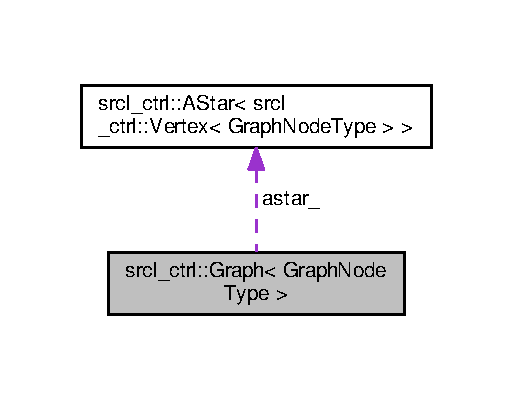
\includegraphics[width=220pt]{classsrcl__ctrl_1_1Graph__coll__graph}
\end{center}
\end{figure}
\subsection*{Public Member Functions}
\begin{DoxyCompactItemize}
\item 
\hyperlink{classsrcl__ctrl_1_1Graph_a0899e8a7a595c50ebd6e33af77be4658}{Graph} ()
\begin{DoxyCompactList}\small\item\em \hyperlink{classsrcl__ctrl_1_1Graph}{Graph} constructor. \end{DoxyCompactList}\item 
\hyperlink{classsrcl__ctrl_1_1Graph_af3e550a78cd615839f10369e9cdd3141}{$\sim$\-Graph} ()
\begin{DoxyCompactList}\small\item\em \hyperlink{classsrcl__ctrl_1_1Graph}{Graph} destructor. \end{DoxyCompactList}\item 
void \hyperlink{classsrcl__ctrl_1_1Graph_ad49ef1a9501f2c58d3cacb5a5c3ca7f1}{Add\-Edge} (const Bundled\-Struct\-Type \&src\-\_\-node, const Bundled\-Struct\-Type \&dst\-\_\-node, double cost)
\begin{DoxyCompactList}\small\item\em This function is used to create a graph by adding edges connecting two nodes. \end{DoxyCompactList}\item 
std\-::vector$<$ \hyperlink{classsrcl__ctrl_1_1Vertex}{Vertex}\\*
$<$ Bundled\-Struct\-Type $>$ $\ast$ $>$ \hyperlink{classsrcl__ctrl_1_1Graph_aff39367003a9f9f5e87c14342b0a5307}{Get\-Graph\-Vertices} ()
\begin{DoxyCompactList}\small\item\em This functions is used to access all vertices of a graph. \end{DoxyCompactList}\item 
std\-::vector$<$ \hyperlink{classsrcl__ctrl_1_1Edge}{Edge}$<$ \hyperlink{classsrcl__ctrl_1_1Vertex}{Vertex}\\*
$<$ Bundled\-Struct\-Type $>$ $>$ $>$ \hyperlink{classsrcl__ctrl_1_1Graph_aeaa992f45305eb658c4fef18d1050064}{Get\-Graph\-Edges} ()
\begin{DoxyCompactList}\small\item\em This functions is used to access all edges of a graph. \end{DoxyCompactList}\item 
\hyperlink{classsrcl__ctrl_1_1Vertex}{Vertex}$<$ Bundled\-Struct\-Type $>$ $\ast$ \hyperlink{classsrcl__ctrl_1_1Graph_a9fa6ba62e45c9a67109f9fe2f27eda86}{Get\-Vertex\-From\-I\-D} (uint64\-\_\-t vertex\-\_\-id)
\begin{DoxyCompactList}\small\item\em This function return the vertex with specified id. \end{DoxyCompactList}\item 
std\-::vector$<$ \hyperlink{classsrcl__ctrl_1_1Vertex}{Vertex}\\*
$<$ Bundled\-Struct\-Type $>$ $\ast$ $>$ \hyperlink{classsrcl__ctrl_1_1Graph_a8ffd8ddc00dc90d53713090d90e7974a}{A\-Star\-Search} (\hyperlink{classsrcl__ctrl_1_1Vertex}{Vertex}$<$ Bundled\-Struct\-Type $>$ $\ast$start, \hyperlink{classsrcl__ctrl_1_1Vertex}{Vertex}$<$ Bundled\-Struct\-Type $>$ $\ast$goal)
\begin{DoxyCompactList}\small\item\em Perform A$\ast$ Search and return a path represented by a serious of vertices. \end{DoxyCompactList}\end{DoxyCompactItemize}
\subsection*{Private Member Functions}
\begin{DoxyCompactItemize}
\item 
\hyperlink{classsrcl__ctrl_1_1Vertex}{Vertex}$<$ Bundled\-Struct\-Type $>$ $\ast$ \hyperlink{classsrcl__ctrl_1_1Graph_ad7d00e1136a82de0d2d76e16f4b467a2}{Get\-Vertex} (const Bundled\-Struct\-Type \&vertex\-\_\-node)
\begin{DoxyCompactList}\small\item\em This function checks if a vertex already exists in the graph. \end{DoxyCompactList}\item 
void \hyperlink{classsrcl__ctrl_1_1Graph_ad616e7b44b7c5a53f3d669b91a083d3e}{Reset\-Graph\-Vertices} ()
\begin{DoxyCompactList}\small\item\em This function is used to reset the vertices for a new search. \end{DoxyCompactList}\end{DoxyCompactItemize}
\subsection*{Private Attributes}
\begin{DoxyCompactItemize}
\item 
std\-::map$<$ uint64\-\_\-t, \hyperlink{classsrcl__ctrl_1_1Vertex}{Vertex}\\*
$<$ Bundled\-Struct\-Type $>$ $\ast$ $>$ \hyperlink{classsrcl__ctrl_1_1Graph_acbd662b725ae169caef9d70b36b74dd1}{vertex\-\_\-map\-\_\-}
\item 
\hyperlink{classsrcl__ctrl_1_1AStar}{A\-Star}$<$ \hyperlink{classsrcl__ctrl_1_1Vertex}{Vertex}\\*
$<$ Bundled\-Struct\-Type $>$ $>$ \hyperlink{classsrcl__ctrl_1_1Graph_a854e80856a38633186bca104eafe209b}{astar\-\_\-}
\end{DoxyCompactItemize}


\subsection{Detailed Description}
\subsubsection*{template$<$typename Bundled\-Struct\-Type$>$class srcl\-\_\-ctrl\-::\-Graph$<$ Bundled\-Struct\-Type $>$}

A graph data structure template. 

\subsection{Constructor \& Destructor Documentation}
\hypertarget{classsrcl__ctrl_1_1Graph_a0899e8a7a595c50ebd6e33af77be4658}{\index{srcl\-\_\-ctrl\-::\-Graph@{srcl\-\_\-ctrl\-::\-Graph}!Graph@{Graph}}
\index{Graph@{Graph}!srcl_ctrl::Graph@{srcl\-\_\-ctrl\-::\-Graph}}
\subsubsection[{Graph}]{\setlength{\rightskip}{0pt plus 5cm}template$<$typename Bundled\-Struct\-Type $>$ {\bf srcl\-\_\-ctrl\-::\-Graph}$<$ Bundled\-Struct\-Type $>$\-::{\bf Graph} (
\begin{DoxyParamCaption}
{}
\end{DoxyParamCaption}
)\hspace{0.3cm}{\ttfamily [inline]}}}\label{classsrcl__ctrl_1_1Graph_a0899e8a7a595c50ebd6e33af77be4658}


\hyperlink{classsrcl__ctrl_1_1Graph}{Graph} constructor. 

\hypertarget{classsrcl__ctrl_1_1Graph_af3e550a78cd615839f10369e9cdd3141}{\index{srcl\-\_\-ctrl\-::\-Graph@{srcl\-\_\-ctrl\-::\-Graph}!$\sim$\-Graph@{$\sim$\-Graph}}
\index{$\sim$\-Graph@{$\sim$\-Graph}!srcl_ctrl::Graph@{srcl\-\_\-ctrl\-::\-Graph}}
\subsubsection[{$\sim$\-Graph}]{\setlength{\rightskip}{0pt plus 5cm}template$<$typename Bundled\-Struct\-Type $>$ {\bf srcl\-\_\-ctrl\-::\-Graph}$<$ Bundled\-Struct\-Type $>$\-::$\sim${\bf Graph} (
\begin{DoxyParamCaption}
{}
\end{DoxyParamCaption}
)\hspace{0.3cm}{\ttfamily [inline]}}}\label{classsrcl__ctrl_1_1Graph_af3e550a78cd615839f10369e9cdd3141}


\hyperlink{classsrcl__ctrl_1_1Graph}{Graph} destructor. 

\hyperlink{classsrcl__ctrl_1_1Graph}{Graph} class is only responsible for the memory recycling of \hyperlink{classsrcl__ctrl_1_1Vertex}{Vertex} and \hyperlink{classsrcl__ctrl_1_1Edge}{Edge} objects. The node, such as a quadtree node or a square cell, which each vertex is associated with needs to be recycled separately, for example by the quadtree/square\-\_\-grid class. 

\subsection{Member Function Documentation}
\hypertarget{classsrcl__ctrl_1_1Graph_ad49ef1a9501f2c58d3cacb5a5c3ca7f1}{\index{srcl\-\_\-ctrl\-::\-Graph@{srcl\-\_\-ctrl\-::\-Graph}!Add\-Edge@{Add\-Edge}}
\index{Add\-Edge@{Add\-Edge}!srcl_ctrl::Graph@{srcl\-\_\-ctrl\-::\-Graph}}
\subsubsection[{Add\-Edge}]{\setlength{\rightskip}{0pt plus 5cm}template$<$typename Bundled\-Struct\-Type $>$ void {\bf srcl\-\_\-ctrl\-::\-Graph}$<$ Bundled\-Struct\-Type $>$\-::Add\-Edge (
\begin{DoxyParamCaption}
\item[{const Bundled\-Struct\-Type \&}]{src\-\_\-node, }
\item[{const Bundled\-Struct\-Type \&}]{dst\-\_\-node, }
\item[{double}]{cost}
\end{DoxyParamCaption}
)\hspace{0.3cm}{\ttfamily [inline]}}}\label{classsrcl__ctrl_1_1Graph_ad49ef1a9501f2c58d3cacb5a5c3ca7f1}


This function is used to create a graph by adding edges connecting two nodes. 

\hypertarget{classsrcl__ctrl_1_1Graph_a8ffd8ddc00dc90d53713090d90e7974a}{\index{srcl\-\_\-ctrl\-::\-Graph@{srcl\-\_\-ctrl\-::\-Graph}!A\-Star\-Search@{A\-Star\-Search}}
\index{A\-Star\-Search@{A\-Star\-Search}!srcl_ctrl::Graph@{srcl\-\_\-ctrl\-::\-Graph}}
\subsubsection[{A\-Star\-Search}]{\setlength{\rightskip}{0pt plus 5cm}template$<$typename Bundled\-Struct\-Type $>$ std\-::vector$<${\bf Vertex}$<$Bundled\-Struct\-Type$>$$\ast$$>$ {\bf srcl\-\_\-ctrl\-::\-Graph}$<$ Bundled\-Struct\-Type $>$\-::A\-Star\-Search (
\begin{DoxyParamCaption}
\item[{{\bf Vertex}$<$ Bundled\-Struct\-Type $>$ $\ast$}]{start, }
\item[{{\bf Vertex}$<$ Bundled\-Struct\-Type $>$ $\ast$}]{goal}
\end{DoxyParamCaption}
)\hspace{0.3cm}{\ttfamily [inline]}}}\label{classsrcl__ctrl_1_1Graph_a8ffd8ddc00dc90d53713090d90e7974a}


Perform A$\ast$ Search and return a path represented by a serious of vertices. 

\hypertarget{classsrcl__ctrl_1_1Graph_aeaa992f45305eb658c4fef18d1050064}{\index{srcl\-\_\-ctrl\-::\-Graph@{srcl\-\_\-ctrl\-::\-Graph}!Get\-Graph\-Edges@{Get\-Graph\-Edges}}
\index{Get\-Graph\-Edges@{Get\-Graph\-Edges}!srcl_ctrl::Graph@{srcl\-\_\-ctrl\-::\-Graph}}
\subsubsection[{Get\-Graph\-Edges}]{\setlength{\rightskip}{0pt plus 5cm}template$<$typename Bundled\-Struct\-Type $>$ std\-::vector$<${\bf Edge}$<${\bf Vertex}$<$Bundled\-Struct\-Type$>$ $>$ $>$ {\bf srcl\-\_\-ctrl\-::\-Graph}$<$ Bundled\-Struct\-Type $>$\-::Get\-Graph\-Edges (
\begin{DoxyParamCaption}
{}
\end{DoxyParamCaption}
)\hspace{0.3cm}{\ttfamily [inline]}}}\label{classsrcl__ctrl_1_1Graph_aeaa992f45305eb658c4fef18d1050064}


This functions is used to access all edges of a graph. 

\hypertarget{classsrcl__ctrl_1_1Graph_aff39367003a9f9f5e87c14342b0a5307}{\index{srcl\-\_\-ctrl\-::\-Graph@{srcl\-\_\-ctrl\-::\-Graph}!Get\-Graph\-Vertices@{Get\-Graph\-Vertices}}
\index{Get\-Graph\-Vertices@{Get\-Graph\-Vertices}!srcl_ctrl::Graph@{srcl\-\_\-ctrl\-::\-Graph}}
\subsubsection[{Get\-Graph\-Vertices}]{\setlength{\rightskip}{0pt plus 5cm}template$<$typename Bundled\-Struct\-Type $>$ std\-::vector$<${\bf Vertex}$<$Bundled\-Struct\-Type$>$$\ast$$>$ {\bf srcl\-\_\-ctrl\-::\-Graph}$<$ Bundled\-Struct\-Type $>$\-::Get\-Graph\-Vertices (
\begin{DoxyParamCaption}
{}
\end{DoxyParamCaption}
)\hspace{0.3cm}{\ttfamily [inline]}}}\label{classsrcl__ctrl_1_1Graph_aff39367003a9f9f5e87c14342b0a5307}


This functions is used to access all vertices of a graph. 

\hypertarget{classsrcl__ctrl_1_1Graph_ad7d00e1136a82de0d2d76e16f4b467a2}{\index{srcl\-\_\-ctrl\-::\-Graph@{srcl\-\_\-ctrl\-::\-Graph}!Get\-Vertex@{Get\-Vertex}}
\index{Get\-Vertex@{Get\-Vertex}!srcl_ctrl::Graph@{srcl\-\_\-ctrl\-::\-Graph}}
\subsubsection[{Get\-Vertex}]{\setlength{\rightskip}{0pt plus 5cm}template$<$typename Bundled\-Struct\-Type $>$ {\bf Vertex}$<$Bundled\-Struct\-Type$>$$\ast$ {\bf srcl\-\_\-ctrl\-::\-Graph}$<$ Bundled\-Struct\-Type $>$\-::Get\-Vertex (
\begin{DoxyParamCaption}
\item[{const Bundled\-Struct\-Type \&}]{vertex\-\_\-node}
\end{DoxyParamCaption}
)\hspace{0.3cm}{\ttfamily [inline]}, {\ttfamily [private]}}}\label{classsrcl__ctrl_1_1Graph_ad7d00e1136a82de0d2d76e16f4b467a2}


This function checks if a vertex already exists in the graph. 

If yes, the functions returns the index of the existing vertex, otherwise it creates a new vertex. \hypertarget{classsrcl__ctrl_1_1Graph_a9fa6ba62e45c9a67109f9fe2f27eda86}{\index{srcl\-\_\-ctrl\-::\-Graph@{srcl\-\_\-ctrl\-::\-Graph}!Get\-Vertex\-From\-I\-D@{Get\-Vertex\-From\-I\-D}}
\index{Get\-Vertex\-From\-I\-D@{Get\-Vertex\-From\-I\-D}!srcl_ctrl::Graph@{srcl\-\_\-ctrl\-::\-Graph}}
\subsubsection[{Get\-Vertex\-From\-I\-D}]{\setlength{\rightskip}{0pt plus 5cm}template$<$typename Bundled\-Struct\-Type $>$ {\bf Vertex}$<$Bundled\-Struct\-Type$>$$\ast$ {\bf srcl\-\_\-ctrl\-::\-Graph}$<$ Bundled\-Struct\-Type $>$\-::Get\-Vertex\-From\-I\-D (
\begin{DoxyParamCaption}
\item[{uint64\-\_\-t}]{vertex\-\_\-id}
\end{DoxyParamCaption}
)\hspace{0.3cm}{\ttfamily [inline]}}}\label{classsrcl__ctrl_1_1Graph_a9fa6ba62e45c9a67109f9fe2f27eda86}


This function return the vertex with specified id. 

\hypertarget{classsrcl__ctrl_1_1Graph_ad616e7b44b7c5a53f3d669b91a083d3e}{\index{srcl\-\_\-ctrl\-::\-Graph@{srcl\-\_\-ctrl\-::\-Graph}!Reset\-Graph\-Vertices@{Reset\-Graph\-Vertices}}
\index{Reset\-Graph\-Vertices@{Reset\-Graph\-Vertices}!srcl_ctrl::Graph@{srcl\-\_\-ctrl\-::\-Graph}}
\subsubsection[{Reset\-Graph\-Vertices}]{\setlength{\rightskip}{0pt plus 5cm}template$<$typename Bundled\-Struct\-Type $>$ void {\bf srcl\-\_\-ctrl\-::\-Graph}$<$ Bundled\-Struct\-Type $>$\-::Reset\-Graph\-Vertices (
\begin{DoxyParamCaption}
{}
\end{DoxyParamCaption}
)\hspace{0.3cm}{\ttfamily [inline]}, {\ttfamily [private]}}}\label{classsrcl__ctrl_1_1Graph_ad616e7b44b7c5a53f3d669b91a083d3e}


This function is used to reset the vertices for a new search. 



\subsection{Member Data Documentation}
\hypertarget{classsrcl__ctrl_1_1Graph_a854e80856a38633186bca104eafe209b}{\index{srcl\-\_\-ctrl\-::\-Graph@{srcl\-\_\-ctrl\-::\-Graph}!astar\-\_\-@{astar\-\_\-}}
\index{astar\-\_\-@{astar\-\_\-}!srcl_ctrl::Graph@{srcl\-\_\-ctrl\-::\-Graph}}
\subsubsection[{astar\-\_\-}]{\setlength{\rightskip}{0pt plus 5cm}template$<$typename Bundled\-Struct\-Type $>$ {\bf A\-Star}$<${\bf Vertex}$<$Bundled\-Struct\-Type$>$ $>$ {\bf srcl\-\_\-ctrl\-::\-Graph}$<$ Bundled\-Struct\-Type $>$\-::astar\-\_\-\hspace{0.3cm}{\ttfamily [private]}}}\label{classsrcl__ctrl_1_1Graph_a854e80856a38633186bca104eafe209b}
\hypertarget{classsrcl__ctrl_1_1Graph_acbd662b725ae169caef9d70b36b74dd1}{\index{srcl\-\_\-ctrl\-::\-Graph@{srcl\-\_\-ctrl\-::\-Graph}!vertex\-\_\-map\-\_\-@{vertex\-\_\-map\-\_\-}}
\index{vertex\-\_\-map\-\_\-@{vertex\-\_\-map\-\_\-}!srcl_ctrl::Graph@{srcl\-\_\-ctrl\-::\-Graph}}
\subsubsection[{vertex\-\_\-map\-\_\-}]{\setlength{\rightskip}{0pt plus 5cm}template$<$typename Bundled\-Struct\-Type $>$ std\-::map$<$uint64\-\_\-t, {\bf Vertex}$<$Bundled\-Struct\-Type$>$$\ast$$>$ {\bf srcl\-\_\-ctrl\-::\-Graph}$<$ Bundled\-Struct\-Type $>$\-::vertex\-\_\-map\-\_\-\hspace{0.3cm}{\ttfamily [private]}}}\label{classsrcl__ctrl_1_1Graph_acbd662b725ae169caef9d70b36b74dd1}


The documentation for this class was generated from the following file\-:\begin{DoxyCompactItemize}
\item 
/home/rdu/\-Workspace/srcl\-\_\-robot\-\_\-suite/srcl\-\_\-ctrl/planning/src/graph/\hyperlink{graph_8h}{graph.\-h}\end{DoxyCompactItemize}

\hypertarget{structsrcl__ctrl_1_1PriorityQueue}{\section{srcl\-\_\-ctrl\-:\-:Priority\-Queue$<$ T, Number $>$ Struct Template Reference}
\label{structsrcl__ctrl_1_1PriorityQueue}\index{srcl\-\_\-ctrl\-::\-Priority\-Queue$<$ T, Number $>$@{srcl\-\_\-ctrl\-::\-Priority\-Queue$<$ T, Number $>$}}
}


A simple priority queue structure used as A$\ast$ open list.  




{\ttfamily \#include $<$astar.\-h$>$}

\subsection*{Public Types}
\begin{DoxyCompactItemize}
\item 
typedef std\-::pair$<$ Number, T $>$ \hyperlink{structsrcl__ctrl_1_1PriorityQueue_a13adb99a78e01b3fbf453e6bc5b8ce39}{P\-Q\-Element}
\end{DoxyCompactItemize}
\subsection*{Public Member Functions}
\begin{DoxyCompactItemize}
\item 
bool \hyperlink{structsrcl__ctrl_1_1PriorityQueue_ad36dcefb2ba7a31f1cd9c78353ac87e3}{empty} () const 
\item 
void \hyperlink{structsrcl__ctrl_1_1PriorityQueue_ac96327c955fa10e88699c8325817c892}{put} (T item, Number priority)
\item 
T \hyperlink{structsrcl__ctrl_1_1PriorityQueue_a51ebef251641f5f51768b7ec4ab94a51}{get} ()
\end{DoxyCompactItemize}
\subsection*{Public Attributes}
\begin{DoxyCompactItemize}
\item 
std\-::priority\-\_\-queue$<$ \hyperlink{structsrcl__ctrl_1_1PriorityQueue_a13adb99a78e01b3fbf453e6bc5b8ce39}{P\-Q\-Element}, \\*
std\-::vector$<$ \hyperlink{structsrcl__ctrl_1_1PriorityQueue_a13adb99a78e01b3fbf453e6bc5b8ce39}{P\-Q\-Element} $>$\\*
, std\-::greater$<$ \hyperlink{structsrcl__ctrl_1_1PriorityQueue_a13adb99a78e01b3fbf453e6bc5b8ce39}{P\-Q\-Element} $>$ $>$ \hyperlink{structsrcl__ctrl_1_1PriorityQueue_afd9907537d5a1df02f71e6e0a7806b8f}{elements}
\end{DoxyCompactItemize}


\subsection{Detailed Description}
\subsubsection*{template$<$typename T, typename Number = double$>$struct srcl\-\_\-ctrl\-::\-Priority\-Queue$<$ T, Number $>$}

A simple priority queue structure used as A$\ast$ open list. 

\subsection{Member Typedef Documentation}
\hypertarget{structsrcl__ctrl_1_1PriorityQueue_a13adb99a78e01b3fbf453e6bc5b8ce39}{\index{srcl\-\_\-ctrl\-::\-Priority\-Queue@{srcl\-\_\-ctrl\-::\-Priority\-Queue}!P\-Q\-Element@{P\-Q\-Element}}
\index{P\-Q\-Element@{P\-Q\-Element}!srcl_ctrl::PriorityQueue@{srcl\-\_\-ctrl\-::\-Priority\-Queue}}
\subsubsection[{P\-Q\-Element}]{\setlength{\rightskip}{0pt plus 5cm}template$<$typename T, typename Number = double$>$ typedef std\-::pair$<$Number, T$>$ {\bf srcl\-\_\-ctrl\-::\-Priority\-Queue}$<$ T, Number $>$\-::{\bf P\-Q\-Element}}}\label{structsrcl__ctrl_1_1PriorityQueue_a13adb99a78e01b3fbf453e6bc5b8ce39}


\subsection{Member Function Documentation}
\hypertarget{structsrcl__ctrl_1_1PriorityQueue_ad36dcefb2ba7a31f1cd9c78353ac87e3}{\index{srcl\-\_\-ctrl\-::\-Priority\-Queue@{srcl\-\_\-ctrl\-::\-Priority\-Queue}!empty@{empty}}
\index{empty@{empty}!srcl_ctrl::PriorityQueue@{srcl\-\_\-ctrl\-::\-Priority\-Queue}}
\subsubsection[{empty}]{\setlength{\rightskip}{0pt plus 5cm}template$<$typename T, typename Number = double$>$ bool {\bf srcl\-\_\-ctrl\-::\-Priority\-Queue}$<$ T, Number $>$\-::empty (
\begin{DoxyParamCaption}
{}
\end{DoxyParamCaption}
) const\hspace{0.3cm}{\ttfamily [inline]}}}\label{structsrcl__ctrl_1_1PriorityQueue_ad36dcefb2ba7a31f1cd9c78353ac87e3}
\hypertarget{structsrcl__ctrl_1_1PriorityQueue_a51ebef251641f5f51768b7ec4ab94a51}{\index{srcl\-\_\-ctrl\-::\-Priority\-Queue@{srcl\-\_\-ctrl\-::\-Priority\-Queue}!get@{get}}
\index{get@{get}!srcl_ctrl::PriorityQueue@{srcl\-\_\-ctrl\-::\-Priority\-Queue}}
\subsubsection[{get}]{\setlength{\rightskip}{0pt plus 5cm}template$<$typename T, typename Number = double$>$ T {\bf srcl\-\_\-ctrl\-::\-Priority\-Queue}$<$ T, Number $>$\-::get (
\begin{DoxyParamCaption}
{}
\end{DoxyParamCaption}
)\hspace{0.3cm}{\ttfamily [inline]}}}\label{structsrcl__ctrl_1_1PriorityQueue_a51ebef251641f5f51768b7ec4ab94a51}
\hypertarget{structsrcl__ctrl_1_1PriorityQueue_ac96327c955fa10e88699c8325817c892}{\index{srcl\-\_\-ctrl\-::\-Priority\-Queue@{srcl\-\_\-ctrl\-::\-Priority\-Queue}!put@{put}}
\index{put@{put}!srcl_ctrl::PriorityQueue@{srcl\-\_\-ctrl\-::\-Priority\-Queue}}
\subsubsection[{put}]{\setlength{\rightskip}{0pt plus 5cm}template$<$typename T, typename Number = double$>$ void {\bf srcl\-\_\-ctrl\-::\-Priority\-Queue}$<$ T, Number $>$\-::put (
\begin{DoxyParamCaption}
\item[{T}]{item, }
\item[{Number}]{priority}
\end{DoxyParamCaption}
)\hspace{0.3cm}{\ttfamily [inline]}}}\label{structsrcl__ctrl_1_1PriorityQueue_ac96327c955fa10e88699c8325817c892}


\subsection{Member Data Documentation}
\hypertarget{structsrcl__ctrl_1_1PriorityQueue_afd9907537d5a1df02f71e6e0a7806b8f}{\index{srcl\-\_\-ctrl\-::\-Priority\-Queue@{srcl\-\_\-ctrl\-::\-Priority\-Queue}!elements@{elements}}
\index{elements@{elements}!srcl_ctrl::PriorityQueue@{srcl\-\_\-ctrl\-::\-Priority\-Queue}}
\subsubsection[{elements}]{\setlength{\rightskip}{0pt plus 5cm}template$<$typename T, typename Number = double$>$ std\-::priority\-\_\-queue$<${\bf P\-Q\-Element}, std\-::vector$<${\bf P\-Q\-Element}$>$, std\-::greater$<${\bf P\-Q\-Element}$>$ $>$ {\bf srcl\-\_\-ctrl\-::\-Priority\-Queue}$<$ T, Number $>$\-::elements}}\label{structsrcl__ctrl_1_1PriorityQueue_afd9907537d5a1df02f71e6e0a7806b8f}


The documentation for this struct was generated from the following file\-:\begin{DoxyCompactItemize}
\item 
/home/rdu/\-Workspace/srcl\-\_\-robot\-\_\-suite/srcl\-\_\-ctrl/planning/src/graph/\hyperlink{astar_8h}{astar.\-h}\end{DoxyCompactItemize}

\hypertarget{classsrcl__ctrl_1_1Vertex}{\section{srcl\-\_\-ctrl\-:\-:Vertex$<$ Vertex\-Node\-Type $>$ Class Template Reference}
\label{classsrcl__ctrl_1_1Vertex}\index{srcl\-\_\-ctrl\-::\-Vertex$<$ Vertex\-Node\-Type $>$@{srcl\-\_\-ctrl\-::\-Vertex$<$ Vertex\-Node\-Type $>$}}
}


A vertex data structure template.  




{\ttfamily \#include $<$vertex.\-h$>$}

\subsection*{Public Member Functions}
\begin{DoxyCompactItemize}
\item 
\hyperlink{classsrcl__ctrl_1_1Vertex_af0578f23ded3d8439e87a3f2ae10292d}{Vertex} (Vertex\-Node\-Type $\ast$node=nullptr)
\item 
\hyperlink{classsrcl__ctrl_1_1Vertex_a0cb4745bc480b9efc8d0e502b16fbd52}{$\sim$\-Vertex} ()
\item 
bool \hyperlink{classsrcl__ctrl_1_1Vertex_a39000d2df49bb8bb1c69031cb643f4f8}{operator==} (const \hyperlink{classsrcl__ctrl_1_1Vertex}{Vertex}$<$ Vertex\-Node\-Type $>$ other)
\item 
void \hyperlink{classsrcl__ctrl_1_1Vertex_a0b523a10a2b6d3c6366351614212d6d7}{Clear\-Vertex\-Search\-Info} ()
\item 
double \hyperlink{classsrcl__ctrl_1_1Vertex_ad1bfb0c6db83570111f38239f253d705}{Get\-Edge\-Cost} (\hyperlink{classsrcl__ctrl_1_1Vertex}{Vertex}$<$ Vertex\-Node\-Type $>$ $\ast$dst\-\_\-node)
\end{DoxyCompactItemize}
\subsection*{Public Attributes}
\begin{DoxyCompactItemize}
\item 
Vertex\-Node\-Type $\ast$ \hyperlink{classsrcl__ctrl_1_1Vertex_a8f6a4fe4b4f90da09585d217a45776c0}{node\-\_\-}
\item 
uint64\-\_\-t \hyperlink{classsrcl__ctrl_1_1Vertex_a3603bcc823fb7faf9e6bfa0dcd75d17f}{vertex\-\_\-id\-\_\-}
\item 
std\-::vector$<$ \hyperlink{classsrcl__ctrl_1_1Edge}{Edge}$<$ \hyperlink{classsrcl__ctrl_1_1Vertex}{Vertex}\\*
$<$ Vertex\-Node\-Type $>$ $>$ $>$ \hyperlink{classsrcl__ctrl_1_1Vertex_a70fcde693fe27f0d683edbe61bacf157}{edges\-\_\-}
\item 
bool \hyperlink{classsrcl__ctrl_1_1Vertex_a0df1a1732482d5a18a255c8295ec47db}{is\-\_\-checked\-\_\-}
\item 
bool \hyperlink{classsrcl__ctrl_1_1Vertex_a903aae6844c345082211eef308df0237}{is\-\_\-in\-\_\-openlist\-\_\-}
\item 
double \hyperlink{classsrcl__ctrl_1_1Vertex_a2e160af974d32d2d45c6919834e6c95e}{f\-\_\-astar\-\_\-}
\item 
double \hyperlink{classsrcl__ctrl_1_1Vertex_a3e4031db49e20d962eb01daf9993a491}{g\-\_\-astar\-\_\-}
\item 
double \hyperlink{classsrcl__ctrl_1_1Vertex_a04fbe2b5fc6293e6f4298d1827847f91}{h\-\_\-astar\-\_\-}
\item 
\hyperlink{classsrcl__ctrl_1_1Vertex}{Vertex}$<$ Vertex\-Node\-Type $>$ $\ast$ \hyperlink{classsrcl__ctrl_1_1Vertex_a24423a829a6b5b22a16778c4d3e560fd}{search\-\_\-parent\-\_\-}
\end{DoxyCompactItemize}


\subsection{Detailed Description}
\subsubsection*{template$<$typename Vertex\-Node\-Type$>$class srcl\-\_\-ctrl\-::\-Vertex$<$ Vertex\-Node\-Type $>$}

A vertex data structure template. 

\subsection{Constructor \& Destructor Documentation}
\hypertarget{classsrcl__ctrl_1_1Vertex_af0578f23ded3d8439e87a3f2ae10292d}{\index{srcl\-\_\-ctrl\-::\-Vertex@{srcl\-\_\-ctrl\-::\-Vertex}!Vertex@{Vertex}}
\index{Vertex@{Vertex}!srcl_ctrl::Vertex@{srcl\-\_\-ctrl\-::\-Vertex}}
\subsubsection[{Vertex}]{\setlength{\rightskip}{0pt plus 5cm}template$<$typename Vertex\-Node\-Type$>$ {\bf srcl\-\_\-ctrl\-::\-Vertex}$<$ Vertex\-Node\-Type $>$\-::{\bf Vertex} (
\begin{DoxyParamCaption}
\item[{Vertex\-Node\-Type $\ast$}]{node = {\ttfamily nullptr}}
\end{DoxyParamCaption}
)\hspace{0.3cm}{\ttfamily [inline]}}}\label{classsrcl__ctrl_1_1Vertex_af0578f23ded3d8439e87a3f2ae10292d}
\hypertarget{classsrcl__ctrl_1_1Vertex_a0cb4745bc480b9efc8d0e502b16fbd52}{\index{srcl\-\_\-ctrl\-::\-Vertex@{srcl\-\_\-ctrl\-::\-Vertex}!$\sim$\-Vertex@{$\sim$\-Vertex}}
\index{$\sim$\-Vertex@{$\sim$\-Vertex}!srcl_ctrl::Vertex@{srcl\-\_\-ctrl\-::\-Vertex}}
\subsubsection[{$\sim$\-Vertex}]{\setlength{\rightskip}{0pt plus 5cm}template$<$typename Vertex\-Node\-Type$>$ {\bf srcl\-\_\-ctrl\-::\-Vertex}$<$ Vertex\-Node\-Type $>$\-::$\sim${\bf Vertex} (
\begin{DoxyParamCaption}
{}
\end{DoxyParamCaption}
)\hspace{0.3cm}{\ttfamily [inline]}}}\label{classsrcl__ctrl_1_1Vertex_a0cb4745bc480b9efc8d0e502b16fbd52}


\subsection{Member Function Documentation}
\hypertarget{classsrcl__ctrl_1_1Vertex_a0b523a10a2b6d3c6366351614212d6d7}{\index{srcl\-\_\-ctrl\-::\-Vertex@{srcl\-\_\-ctrl\-::\-Vertex}!Clear\-Vertex\-Search\-Info@{Clear\-Vertex\-Search\-Info}}
\index{Clear\-Vertex\-Search\-Info@{Clear\-Vertex\-Search\-Info}!srcl_ctrl::Vertex@{srcl\-\_\-ctrl\-::\-Vertex}}
\subsubsection[{Clear\-Vertex\-Search\-Info}]{\setlength{\rightskip}{0pt plus 5cm}template$<$typename Vertex\-Node\-Type$>$ void {\bf srcl\-\_\-ctrl\-::\-Vertex}$<$ Vertex\-Node\-Type $>$\-::Clear\-Vertex\-Search\-Info (
\begin{DoxyParamCaption}
{}
\end{DoxyParamCaption}
)\hspace{0.3cm}{\ttfamily [inline]}}}\label{classsrcl__ctrl_1_1Vertex_a0b523a10a2b6d3c6366351614212d6d7}
\hypertarget{classsrcl__ctrl_1_1Vertex_ad1bfb0c6db83570111f38239f253d705}{\index{srcl\-\_\-ctrl\-::\-Vertex@{srcl\-\_\-ctrl\-::\-Vertex}!Get\-Edge\-Cost@{Get\-Edge\-Cost}}
\index{Get\-Edge\-Cost@{Get\-Edge\-Cost}!srcl_ctrl::Vertex@{srcl\-\_\-ctrl\-::\-Vertex}}
\subsubsection[{Get\-Edge\-Cost}]{\setlength{\rightskip}{0pt plus 5cm}template$<$typename Vertex\-Node\-Type$>$ double {\bf srcl\-\_\-ctrl\-::\-Vertex}$<$ Vertex\-Node\-Type $>$\-::Get\-Edge\-Cost (
\begin{DoxyParamCaption}
\item[{{\bf Vertex}$<$ Vertex\-Node\-Type $>$ $\ast$}]{dst\-\_\-node}
\end{DoxyParamCaption}
)\hspace{0.3cm}{\ttfamily [inline]}}}\label{classsrcl__ctrl_1_1Vertex_ad1bfb0c6db83570111f38239f253d705}
\hypertarget{classsrcl__ctrl_1_1Vertex_a39000d2df49bb8bb1c69031cb643f4f8}{\index{srcl\-\_\-ctrl\-::\-Vertex@{srcl\-\_\-ctrl\-::\-Vertex}!operator==@{operator==}}
\index{operator==@{operator==}!srcl_ctrl::Vertex@{srcl\-\_\-ctrl\-::\-Vertex}}
\subsubsection[{operator==}]{\setlength{\rightskip}{0pt plus 5cm}template$<$typename Vertex\-Node\-Type$>$ bool {\bf srcl\-\_\-ctrl\-::\-Vertex}$<$ Vertex\-Node\-Type $>$\-::operator== (
\begin{DoxyParamCaption}
\item[{const {\bf Vertex}$<$ Vertex\-Node\-Type $>$}]{other}
\end{DoxyParamCaption}
)\hspace{0.3cm}{\ttfamily [inline]}}}\label{classsrcl__ctrl_1_1Vertex_a39000d2df49bb8bb1c69031cb643f4f8}


\subsection{Member Data Documentation}
\hypertarget{classsrcl__ctrl_1_1Vertex_a70fcde693fe27f0d683edbe61bacf157}{\index{srcl\-\_\-ctrl\-::\-Vertex@{srcl\-\_\-ctrl\-::\-Vertex}!edges\-\_\-@{edges\-\_\-}}
\index{edges\-\_\-@{edges\-\_\-}!srcl_ctrl::Vertex@{srcl\-\_\-ctrl\-::\-Vertex}}
\subsubsection[{edges\-\_\-}]{\setlength{\rightskip}{0pt plus 5cm}template$<$typename Vertex\-Node\-Type$>$ std\-::vector$<${\bf Edge}$<${\bf Vertex}$<$Vertex\-Node\-Type$>$ $>$ $>$ {\bf srcl\-\_\-ctrl\-::\-Vertex}$<$ Vertex\-Node\-Type $>$\-::edges\-\_\-}}\label{classsrcl__ctrl_1_1Vertex_a70fcde693fe27f0d683edbe61bacf157}
\hypertarget{classsrcl__ctrl_1_1Vertex_a2e160af974d32d2d45c6919834e6c95e}{\index{srcl\-\_\-ctrl\-::\-Vertex@{srcl\-\_\-ctrl\-::\-Vertex}!f\-\_\-astar\-\_\-@{f\-\_\-astar\-\_\-}}
\index{f\-\_\-astar\-\_\-@{f\-\_\-astar\-\_\-}!srcl_ctrl::Vertex@{srcl\-\_\-ctrl\-::\-Vertex}}
\subsubsection[{f\-\_\-astar\-\_\-}]{\setlength{\rightskip}{0pt plus 5cm}template$<$typename Vertex\-Node\-Type$>$ double {\bf srcl\-\_\-ctrl\-::\-Vertex}$<$ Vertex\-Node\-Type $>$\-::f\-\_\-astar\-\_\-}}\label{classsrcl__ctrl_1_1Vertex_a2e160af974d32d2d45c6919834e6c95e}
\hypertarget{classsrcl__ctrl_1_1Vertex_a3e4031db49e20d962eb01daf9993a491}{\index{srcl\-\_\-ctrl\-::\-Vertex@{srcl\-\_\-ctrl\-::\-Vertex}!g\-\_\-astar\-\_\-@{g\-\_\-astar\-\_\-}}
\index{g\-\_\-astar\-\_\-@{g\-\_\-astar\-\_\-}!srcl_ctrl::Vertex@{srcl\-\_\-ctrl\-::\-Vertex}}
\subsubsection[{g\-\_\-astar\-\_\-}]{\setlength{\rightskip}{0pt plus 5cm}template$<$typename Vertex\-Node\-Type$>$ double {\bf srcl\-\_\-ctrl\-::\-Vertex}$<$ Vertex\-Node\-Type $>$\-::g\-\_\-astar\-\_\-}}\label{classsrcl__ctrl_1_1Vertex_a3e4031db49e20d962eb01daf9993a491}
\hypertarget{classsrcl__ctrl_1_1Vertex_a04fbe2b5fc6293e6f4298d1827847f91}{\index{srcl\-\_\-ctrl\-::\-Vertex@{srcl\-\_\-ctrl\-::\-Vertex}!h\-\_\-astar\-\_\-@{h\-\_\-astar\-\_\-}}
\index{h\-\_\-astar\-\_\-@{h\-\_\-astar\-\_\-}!srcl_ctrl::Vertex@{srcl\-\_\-ctrl\-::\-Vertex}}
\subsubsection[{h\-\_\-astar\-\_\-}]{\setlength{\rightskip}{0pt plus 5cm}template$<$typename Vertex\-Node\-Type$>$ double {\bf srcl\-\_\-ctrl\-::\-Vertex}$<$ Vertex\-Node\-Type $>$\-::h\-\_\-astar\-\_\-}}\label{classsrcl__ctrl_1_1Vertex_a04fbe2b5fc6293e6f4298d1827847f91}
\hypertarget{classsrcl__ctrl_1_1Vertex_a0df1a1732482d5a18a255c8295ec47db}{\index{srcl\-\_\-ctrl\-::\-Vertex@{srcl\-\_\-ctrl\-::\-Vertex}!is\-\_\-checked\-\_\-@{is\-\_\-checked\-\_\-}}
\index{is\-\_\-checked\-\_\-@{is\-\_\-checked\-\_\-}!srcl_ctrl::Vertex@{srcl\-\_\-ctrl\-::\-Vertex}}
\subsubsection[{is\-\_\-checked\-\_\-}]{\setlength{\rightskip}{0pt plus 5cm}template$<$typename Vertex\-Node\-Type$>$ bool {\bf srcl\-\_\-ctrl\-::\-Vertex}$<$ Vertex\-Node\-Type $>$\-::is\-\_\-checked\-\_\-}}\label{classsrcl__ctrl_1_1Vertex_a0df1a1732482d5a18a255c8295ec47db}
\hypertarget{classsrcl__ctrl_1_1Vertex_a903aae6844c345082211eef308df0237}{\index{srcl\-\_\-ctrl\-::\-Vertex@{srcl\-\_\-ctrl\-::\-Vertex}!is\-\_\-in\-\_\-openlist\-\_\-@{is\-\_\-in\-\_\-openlist\-\_\-}}
\index{is\-\_\-in\-\_\-openlist\-\_\-@{is\-\_\-in\-\_\-openlist\-\_\-}!srcl_ctrl::Vertex@{srcl\-\_\-ctrl\-::\-Vertex}}
\subsubsection[{is\-\_\-in\-\_\-openlist\-\_\-}]{\setlength{\rightskip}{0pt plus 5cm}template$<$typename Vertex\-Node\-Type$>$ bool {\bf srcl\-\_\-ctrl\-::\-Vertex}$<$ Vertex\-Node\-Type $>$\-::is\-\_\-in\-\_\-openlist\-\_\-}}\label{classsrcl__ctrl_1_1Vertex_a903aae6844c345082211eef308df0237}
\hypertarget{classsrcl__ctrl_1_1Vertex_a8f6a4fe4b4f90da09585d217a45776c0}{\index{srcl\-\_\-ctrl\-::\-Vertex@{srcl\-\_\-ctrl\-::\-Vertex}!node\-\_\-@{node\-\_\-}}
\index{node\-\_\-@{node\-\_\-}!srcl_ctrl::Vertex@{srcl\-\_\-ctrl\-::\-Vertex}}
\subsubsection[{node\-\_\-}]{\setlength{\rightskip}{0pt plus 5cm}template$<$typename Vertex\-Node\-Type$>$ Vertex\-Node\-Type$\ast$ {\bf srcl\-\_\-ctrl\-::\-Vertex}$<$ Vertex\-Node\-Type $>$\-::node\-\_\-}}\label{classsrcl__ctrl_1_1Vertex_a8f6a4fe4b4f90da09585d217a45776c0}
\hypertarget{classsrcl__ctrl_1_1Vertex_a24423a829a6b5b22a16778c4d3e560fd}{\index{srcl\-\_\-ctrl\-::\-Vertex@{srcl\-\_\-ctrl\-::\-Vertex}!search\-\_\-parent\-\_\-@{search\-\_\-parent\-\_\-}}
\index{search\-\_\-parent\-\_\-@{search\-\_\-parent\-\_\-}!srcl_ctrl::Vertex@{srcl\-\_\-ctrl\-::\-Vertex}}
\subsubsection[{search\-\_\-parent\-\_\-}]{\setlength{\rightskip}{0pt plus 5cm}template$<$typename Vertex\-Node\-Type$>$ {\bf Vertex}$<$Vertex\-Node\-Type$>$$\ast$ {\bf srcl\-\_\-ctrl\-::\-Vertex}$<$ Vertex\-Node\-Type $>$\-::search\-\_\-parent\-\_\-}}\label{classsrcl__ctrl_1_1Vertex_a24423a829a6b5b22a16778c4d3e560fd}
\hypertarget{classsrcl__ctrl_1_1Vertex_a3603bcc823fb7faf9e6bfa0dcd75d17f}{\index{srcl\-\_\-ctrl\-::\-Vertex@{srcl\-\_\-ctrl\-::\-Vertex}!vertex\-\_\-id\-\_\-@{vertex\-\_\-id\-\_\-}}
\index{vertex\-\_\-id\-\_\-@{vertex\-\_\-id\-\_\-}!srcl_ctrl::Vertex@{srcl\-\_\-ctrl\-::\-Vertex}}
\subsubsection[{vertex\-\_\-id\-\_\-}]{\setlength{\rightskip}{0pt plus 5cm}template$<$typename Vertex\-Node\-Type$>$ uint64\-\_\-t {\bf srcl\-\_\-ctrl\-::\-Vertex}$<$ Vertex\-Node\-Type $>$\-::vertex\-\_\-id\-\_\-}}\label{classsrcl__ctrl_1_1Vertex_a3603bcc823fb7faf9e6bfa0dcd75d17f}


The documentation for this class was generated from the following file\-:\begin{DoxyCompactItemize}
\item 
/home/rdu/\-Workspace/srcl\-\_\-robot\-\_\-suite/srcl\-\_\-ctrl/planning/src/graph/\hyperlink{vertex_8h}{vertex.\-h}\end{DoxyCompactItemize}

\chapter{File Documentation}
\hypertarget{graph_8md}{\section{graph.\-md File Reference}
\label{graph_8md}\index{graph.\-md@{graph.\-md}}
}

\hypertarget{known__issues_8md}{\section{known\-\_\-issues.\-md File Reference}
\label{known__issues_8md}\index{known\-\_\-issues.\-md@{known\-\_\-issues.\-md}}
}

\hypertarget{mainpage_8md}{\section{mainpage.\-md File Reference}
\label{mainpage_8md}\index{mainpage.\-md@{mainpage.\-md}}
}

\hypertarget{astar_8h}{\section{/home/rdu/\-Workspace/srcl\-\_\-robot\-\_\-suite/srcl\-\_\-ctrl/planning/src/graph/astar.h File Reference}
\label{astar_8h}\index{/home/rdu/\-Workspace/srcl\-\_\-robot\-\_\-suite/srcl\-\_\-ctrl/planning/src/graph/astar.\-h@{/home/rdu/\-Workspace/srcl\-\_\-robot\-\_\-suite/srcl\-\_\-ctrl/planning/src/graph/astar.\-h}}
}
{\ttfamily \#include $<$vector$>$}\\*
{\ttfamily \#include $<$queue$>$}\\*
{\ttfamily \#include $<$functional$>$}\\*
{\ttfamily \#include $<$utility$>$}\\*
{\ttfamily \#include $<$cmath$>$}\\*
{\ttfamily \#include $<$algorithm$>$}\\*
{\ttfamily \#include $<$vertex.\-h$>$}\\*
Include dependency graph for astar.\-h\-:\nopagebreak
\begin{figure}[H]
\begin{center}
\leavevmode
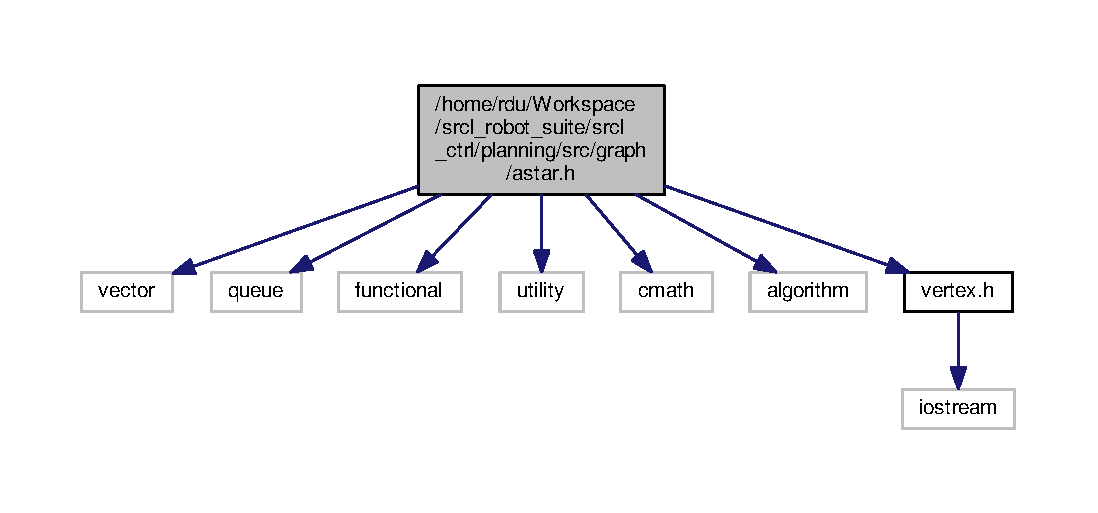
\includegraphics[width=350pt]{astar_8h__incl}
\end{center}
\end{figure}
This graph shows which files directly or indirectly include this file\-:\nopagebreak
\begin{figure}[H]
\begin{center}
\leavevmode
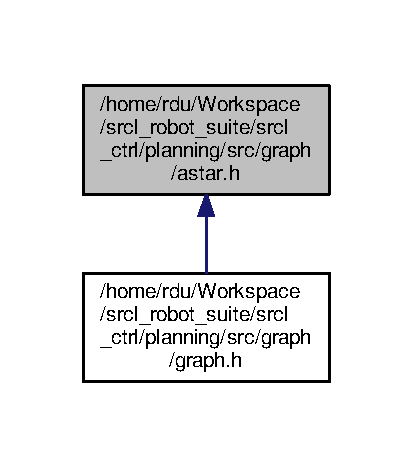
\includegraphics[width=198pt]{astar_8h__dep__incl}
\end{center}
\end{figure}
\subsection*{Classes}
\begin{DoxyCompactItemize}
\item 
struct \hyperlink{structsrcl__ctrl_1_1PriorityQueue}{srcl\-\_\-ctrl\-::\-Priority\-Queue$<$ T, Number $>$}
\begin{DoxyCompactList}\small\item\em A simple priority queue structure used as A$\ast$ open list. \end{DoxyCompactList}\item 
class \hyperlink{classsrcl__ctrl_1_1AStar}{srcl\-\_\-ctrl\-::\-A\-Star$<$ Graph\-Vertex\-Type $>$}
\begin{DoxyCompactList}\small\item\em A$\ast$ search algorithm. \end{DoxyCompactList}\end{DoxyCompactItemize}
\subsection*{Namespaces}
\begin{DoxyCompactItemize}
\item 
\hyperlink{namespacesrcl__ctrl}{srcl\-\_\-ctrl}
\end{DoxyCompactItemize}

\hypertarget{graph_8h}{\section{/home/rdu/\-Workspace/srcl\-\_\-robot\-\_\-suite/srcl\-\_\-ctrl/planning/src/graph/graph.h File Reference}
\label{graph_8h}\index{/home/rdu/\-Workspace/srcl\-\_\-robot\-\_\-suite/srcl\-\_\-ctrl/planning/src/graph/graph.\-h@{/home/rdu/\-Workspace/srcl\-\_\-robot\-\_\-suite/srcl\-\_\-ctrl/planning/src/graph/graph.\-h}}
}
{\ttfamily \#include $<$map$>$}\\*
{\ttfamily \#include $<$vector$>$}\\*
{\ttfamily \#include $<$cstdint$>$}\\*
{\ttfamily \#include $<$vertex.\-h$>$}\\*
{\ttfamily \#include $<$astar.\-h$>$}\\*
Include dependency graph for graph.\-h\-:\nopagebreak
\begin{figure}[H]
\begin{center}
\leavevmode
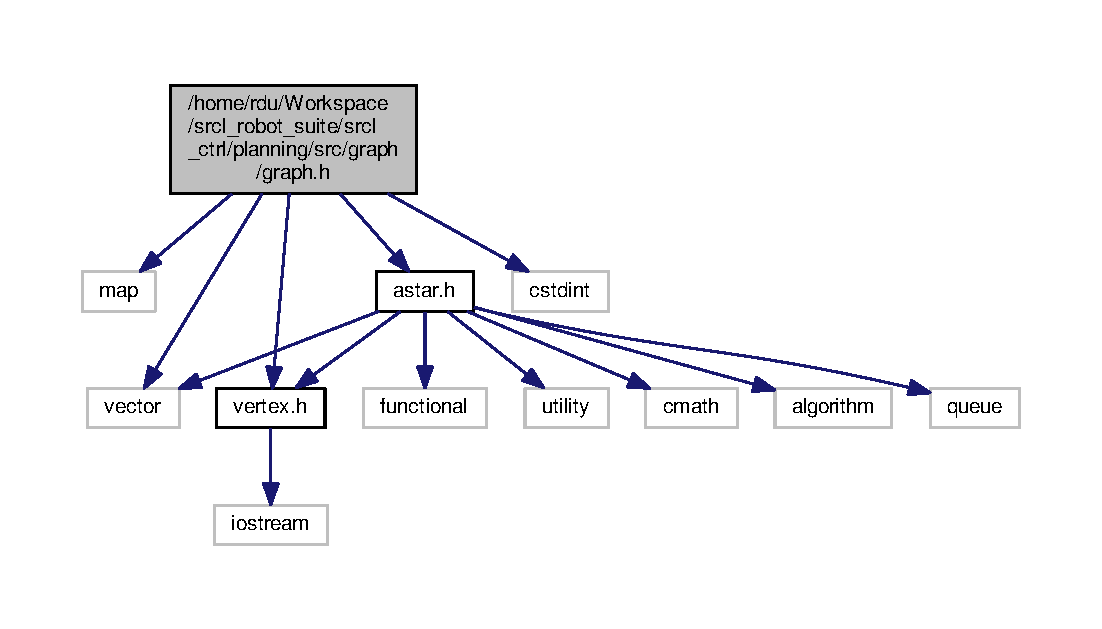
\includegraphics[width=350pt]{graph_8h__incl}
\end{center}
\end{figure}
\subsection*{Classes}
\begin{DoxyCompactItemize}
\item 
struct \hyperlink{structsrcl__ctrl_1_1ExampleNode}{srcl\-\_\-ctrl\-::\-Example\-Node}
\begin{DoxyCompactList}\small\item\em An example node that can be associated with a vertex. \end{DoxyCompactList}\item 
class \hyperlink{classsrcl__ctrl_1_1Graph}{srcl\-\_\-ctrl\-::\-Graph$<$ Graph\-Node\-Type $>$}
\begin{DoxyCompactList}\small\item\em A graph data structure template. \end{DoxyCompactList}\end{DoxyCompactItemize}
\subsection*{Namespaces}
\begin{DoxyCompactItemize}
\item 
\hyperlink{namespacesrcl__ctrl}{srcl\-\_\-ctrl}
\end{DoxyCompactItemize}

\hypertarget{README_8md}{\section{/home/rdu/\-Workspace/srcl\-\_\-robot\-\_\-suite/srcl\-\_\-ctrl/planning/src/graph/\-R\-E\-A\-D\-M\-E.md File Reference}
\label{README_8md}\index{/home/rdu/\-Workspace/srcl\-\_\-robot\-\_\-suite/srcl\-\_\-ctrl/planning/src/graph/\-R\-E\-A\-D\-M\-E.\-md@{/home/rdu/\-Workspace/srcl\-\_\-robot\-\_\-suite/srcl\-\_\-ctrl/planning/src/graph/\-R\-E\-A\-D\-M\-E.\-md}}
}

\hypertarget{vertex_8h}{\section{/home/rdu/\-Workspace/srcl\-\_\-robot\-\_\-suite/srcl\-\_\-ctrl/planning/src/graph/vertex.h File Reference}
\label{vertex_8h}\index{/home/rdu/\-Workspace/srcl\-\_\-robot\-\_\-suite/srcl\-\_\-ctrl/planning/src/graph/vertex.\-h@{/home/rdu/\-Workspace/srcl\-\_\-robot\-\_\-suite/srcl\-\_\-ctrl/planning/src/graph/vertex.\-h}}
}
{\ttfamily \#include $<$iostream$>$}\\*
Include dependency graph for vertex.\-h\-:\nopagebreak
\begin{figure}[H]
\begin{center}
\leavevmode
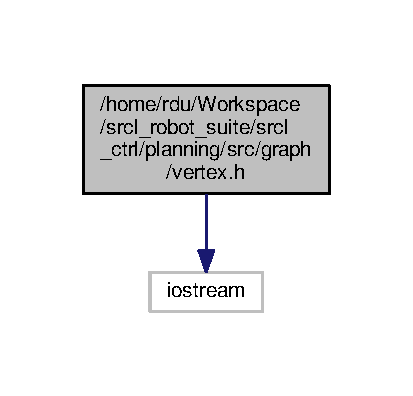
\includegraphics[width=198pt]{vertex_8h__incl}
\end{center}
\end{figure}
This graph shows which files directly or indirectly include this file\-:\nopagebreak
\begin{figure}[H]
\begin{center}
\leavevmode
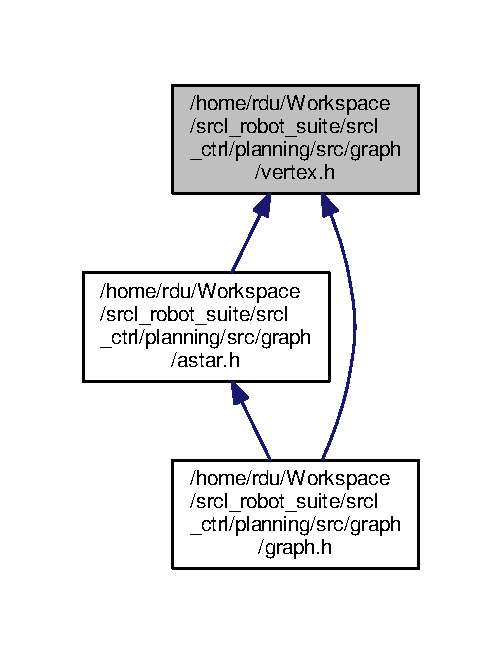
\includegraphics[width=241pt]{vertex_8h__dep__incl}
\end{center}
\end{figure}
\subsection*{Classes}
\begin{DoxyCompactItemize}
\item 
class \hyperlink{classsrcl__ctrl_1_1Edge}{srcl\-\_\-ctrl\-::\-Edge$<$ Bundled\-Vertex\-Type $>$}
\begin{DoxyCompactList}\small\item\em An edge data structure template. \end{DoxyCompactList}\item 
class \hyperlink{classsrcl__ctrl_1_1Vertex}{srcl\-\_\-ctrl\-::\-Vertex$<$ Bundled\-Struct\-Type $>$}
\begin{DoxyCompactList}\small\item\em A vertex data structure template. \end{DoxyCompactList}\end{DoxyCompactItemize}
\subsection*{Namespaces}
\begin{DoxyCompactItemize}
\item 
\hyperlink{namespacesrcl__ctrl}{srcl\-\_\-ctrl}
\end{DoxyCompactItemize}

%--- End generated contents ---

% Index
\newpage
\phantomsection
\addcontentsline{toc}{chapter}{Index}
\printindex

\end{document}
